\documentclass[11pt,a4paper]{article}
\usepackage[margin=2.5cm]{geometry}
\usepackage{amsmath,amssymb}
\usepackage{graphicx}
\usepackage[export]{adjustbox}
\usepackage{booktabs}
\usepackage{longtable}
\usepackage{tabularx}
\usepackage{xcolor}
\usepackage{tcolorbox}
\tcbuselibrary{breakable}
\usepackage{enumitem}
\usepackage{microtype}
\usepackage{needspace}
\usepackage{url}
\urlstyle{tt}
\emergencystretch=2em
\definecolor{labblue}{HTML}{1F4E79}
\widowpenalty=10000
\clubpenalty=10000
\setlength{\parskip}{0.35em}
\usepackage{fontspec}
\setmainfont{Liberation Serif}
\setsansfont{Liberation Sans}
\setmonofont{Liberation Mono}
\usepackage[russian]{babel}
\usepackage[colorlinks=true, linkcolor=labblue,
            citecolor=labblue, urlcolor=labblue, bookmarks=true,
            bookmarksnumbered=true, unicode=true]{hyperref}
\begin{document}
\begin{center}
{\huge\bfseries\color{labblue} Дираковский скелет AB-Cloud}\\[0.8em]
{\large Численная лаборатория, связывающая хофштадтеровско-вихревую реализацию программы Гильберта--Пойа с уравнением Дирака}\\[1.2em]
{\normalsize Исаев Исхак Хамзатович}\\[0.3em]
{\small ORCID 0009-0003-7299-0701 --- Независимый исследователь --- программа AB-Cloud Research}\\[0.3em]
{\small Октябрь 2026}
\end{center}
\begin{tcolorbox}[breakable, colback=labblue!6, colframe=labblue!70!black, boxrule=0.6pt, title={Abstract / Аннотация}]
Программа AB-Cloud в родительском репозитории строит хофштадтеровский гамильтониан, украшенный топологическими вихрями, фазы которых кодируют нетривиальные нули дзета-функции Римана, и подтвердила, что в самодуальной точке потока alpha = 1/2 система демонстрирует дираковскую динамику (E\_\allowbreak{}min пропорционально 1/L, R-квадрат = 0.9997). Настоящая монография развивает это наблюдение в полную решёточно-дираковскую лабораторию из восьми верификационных тестов (D1--D8). Численно доказано, что чистая модель Хофштадтера при alpha = 1/2 ЕСТЬ решёточная дискретизация безмассового уравнения Дирака: блоховские зоны совпадают с аналитической пи-флюкс дисперсией до 2.7e-15, ферми-скорость из финально-размерного скейлинга равна v\_\allowbreak{}F = 1.935 в единицах перескока (континуальный прогноз v\_\allowbreak{}F = 2t, фит родительского сьюта v\_\allowbreak{}F = 1.9447), а первый дираковский уровень подчиняется E\_\allowbreak{}1 x L -> 2*pi*v\_\allowbreak{}F = 4*pi с точностью 0.8 процента. Четырёхкратная башня нулевых мод показана как дираковская структура нулевых мод на торе с точным субрешёточным (киральным) балансом поляризации; петля Вильсона вокруг конуса возвращает фазу Берри gamma = pi с двенадцатью десятичными знаками; однородное отклонение поля порождает релятивистскую лестницу Ландау E\_\allowbreak{}n-квадрат пропорционально n (R-квадрат = 0.99985--0.99999) с киральным уровнем n = 0, приколотым к E = 0, в резком контрасте со шрёдингеровской лестницей E\_\allowbreak{}n = B(n + 1/2) того же контрольного оператора. Симуляции реального времени воспроизводят туннелирование Клейна (прохождение при нормальном падении T = 0.978 через барьер, подавляющий шрёдингеровский контроль до T = 0.0010 --- фактор 977) и цвиттербевегунг на частоте omega = 2E (измерено/теория = 0.99958 в ящике Дирака и 0.9998 на самом торе лаборатории). Мостовой тест D7 украшает дираковскую решётку вихревыми фазами, позиции которых детерминированно закодированы первыми нулями дзеты: киральный скелет выживает точно (\{H, Gamma\} = 0 и парность E <-> -E до 4e-15), статистика отношений уровней сдвигается от GOE-потолка к значению GUE 0.5992 (среднее отношение r: 0.41--0.52 чистая -> 0.605--0.608 декорированная), тогда как точная четырёхбашня распадается на пары +-E по долинам --- честный негативный результат, механизм которого (нулевой индекс, смешивание долин) установлен в тесте D8. Вывод: дираковский оператор --- релятивистский скелет AB-Cloud; фазы нулей дзеты действуют как топологически безопасный комплексификатор, открывающий статистику GUE без разрушения релятивистской структуры, необходимой программе Гильберта--Пойа. Расширения v1.1 реализуют оба направления развития, намеченных в первом издании. Тест D9 (восстановление индекса) показывает: массовая доменная стенка Джекива--Ребби связывает киральные пары квази-нулевых мод, заякоренные в 4$\cdot$10$^{8}$ раз ниже объёмной щели грида-дираковского оператора; мода стенки выживает без изменений в полном дзета-вихревом фоне --- контраст восстановления относительно контроля без стенки достигает 7$\cdot$10$^{6}$; а полный составной вихрь Джекива--Росси (намотка массы $\nu$ плюс статистический голдстоуновский поток $\nu$/2) схлопывает низкоэнергетическое ядро до машинного нуля. Тест D10 (Монтгомери в движении) проверяет парную корреляцию Монтгомери развёрнутой последовательности нулей (g(0,3) = 0,19 против теории 0,26 и пуассоновской единицы; дисперсия числа в 60 раз ниже пуассоновской) и демонстрирует динамически, что отталкивание GUE защищает транспорт: дзета-кодированное вихревое облако отражает меньше всех и пропускает больше всех среди конфигураций равной плотности. Таким образом, дзета-фазы, дираковский скелет и статистика Монтгомери нулей связаны в обоих направлениях: спектр несёт нули, а динамика несёт статистику. Расширение v1.2 реализует последнее из трёх направлений --- кодирование нулей через действие сопряжения в духе Берри--Китинга и Коннеса. Тест D11 строит точную решётчатую реализацию обрезанного оператора дилатации (арифметический спектр с точностью 1,7$\cdot$10$^{-}$$^{1}$$^{3}$, точная алгебра сопряжения, точная гребёнка следов Дирихле периода $\Lambda$), доказывает идентичность распознавания --- кодирующая фаза AB-Cloud t/$\delta$ есть дробная часть лестницы Берри--Китинга с точностью 4,6$\cdot$10$^{-}$$^{1}$$^{3}$ --- проверяет на реальных нулях, что обрезанная лестница следит за счётом Римана с точностью $\pm$2,3 единицы нуля при смещении 7/8 + $\langle$S$\rangle$, показывает, что транспортная защита переживает коннесовскую подстановку кодирующей функции (пропускание в 1,65 раза выше пуассоновского; эквивалентность с исходным кодированием до 1,4\%), и читает нули как спектр поглощения сопрягающего драйва: форм-фактор драйва следует GUE-рампе при $\tau$ $\le$ 0,75, а защищённый транспортный класс сохраняется вдоль всей орбиты дилатации. Все одиннадцать тестов --- 67 проверок --- проходят в каноническом прогоне; операторный блок D11 кросс-верифицирован на Julia. Расширения v1.3 выходят за рамки \S{}8 монографии и закрывают его естественные продолжения. Тест D12 доводит лестницу Берри--Китинга до бесконечного предела при фиксированной спектральной плотности: гребёнка следов заостряется в дельта-поезд формулы следа Коннеса--Вейля (когерентный пик равен N\_\allowbreak{}u точно, вне-пиковая огибающая 1/(N\_\allowbreak{}u$\cdot$sin($\pi$/20)) опускается до 1,9$\cdot$10$^{-}$$^{4}$ при N\_\allowbreak{}u = 32768), лестница фиксированной плотности остаётся точным целочисленным тождеством при любом размере полосы, расширяющаяся полоса поглощает всё окно реальных нулей, а дзета-защита оказывается экстенсивной --- GUE-статистика не зависит от размера решётки при фиксированной плотности вихрей 25/900, пока закодированная лестница растёт от 25 до 64 вихрей. Тест D13 спаривает два предыдущих расширения: стенка Джекива--Росси едет по физической коннесовской орбите заякоренной на |E$_{0}$| = 3,9$\cdot$10$^{-}$$^{9}$ (точность профиля 0,9999, контраст 7$\cdot$10$^{6}$ вдоль всей орбиты), а сопрягающий генератор приподнимает валлейный мультиплет лишь до квази-нулевого полоса на gap/679 --- через явно измеренное нарушение киральности \{H($\lambda$), $\Gamma$\} = $\lambda$\{V, $\Gamma$\}. Тест D14 измеряет второй (двухточечный) форм-фактор по Одлыжко на трёх полосах реальных нулей, включая по-настоящему высоковысотную полосу из 2000 нулей при t \textasciitilde{} 10$^{5}$ из официальной таблицы zeros6: жёсткое ядро K(0,1) $\le$ 0,008, GUE-рампа K(0,25) = 0,123 < K(0,5) = 0,396 и единичное плато уже точное при t \textasciitilde{} 10$^{5}$ (K(2) = 0,962) с честно задокументированными отклонениями (струна оценщика при $\tau$ = 1, полососпецифичный подъём K(0,25)). Все четырнадцать тестов --- 96 проверок --- проходят в каноническом прогоне; блоки D12--D14 кросс-верифицированы на Julia.
\end{tcolorbox}
\tableofcontents
\newpage
\section{1. Введение: от фазового резонатора к уравнению Дирака}
Гипотеза Гильберта--Пойа утверждает, что нетривиальные нули дзета-функции Римана являются спектром некоторого самосопряжённого оператора. Программа AB-Cloud родительского репозитория превращает это утверждение в явную решёточную конструкцию: гамильтониан Хофштадтера на решётке L x L, пронизанный однородным ааронов-бовским потоком alpha на одну ячейку и украшенный топологическими вихрями, заряды и фазы которых выведены из нетривиальных нулей rho\_\allowbreak{}k = 1/2 + i t\_\allowbreak{}k функции zeta(s). Родительский верификационный сьют (37 тестов, два прохода, десять независимых языковых портов) установил, что этот объект воспроизводит статистику GUE, статистически неотличим от самих нулей дзеты в тесте Монтгомери и --- решающее для настоящей работы --- демонстрирует дираковскую динамику в самодуальной точке alpha = 1/2: минимальное возбуждение масштабируется как E\_\allowbreak{}min пропорционально 1/L с R-квадрат = 0.9997, плотность состояний развивает глубокую впадину при нулевой энергии, а четырёхкратная башня нулевых мод сидит при машинно-точном E = 0.

Закон скейлинга E пропорционально 1/L --- неоспоримый отпечаток релятивистской дисперсии. Для массивной (нерелятивистской) частицы низшие уровни в коробке размера L выходят на константу; только линейная дисперсия E = v\_\allowbreak{}F|k| даёт E пропорционально 1/L. Родительский сьют зафиксировал отпечаток, но не распаковал его. Настоящая монография распаковывает его. Мы задаём и количественно отвечаем на четыре вопроса. Во-первых, является ли модель Хофштадтера при alpha = 1/2 точно решёточным уравнением Дирака, и каков её континуальный предел? Во-вторых, каково топологическое содержание её нулевых мод --- защищены ли они и чем? В-третьих, совпадает ли физика реального времени решётки со знаменитыми релятивистскими явлениями --- туннелированием Клейна и цвиттербевегунгом --- количественно? В-четвёртых, центральный для программы AB-Cloud: что происходит с этим дираковским скелетом при украшении фазами нулей дзеты, определяющими AB-cloud?

Ответы доставляет одиннадцатитестовая верификационная серия (D1--D11), написанная в культуре родительского репозитория: однофайловость, минимум зависимостей, детерминизм (зерно 96), явные вердикты PASS/FAIL, артефакты CSV по каждому тесту, публикационные фигуры 600 dpi и полная независимая кросс-реализация на Julia, чьи результаты совпадают с каноническим Python-сьютом с точностью LAPACK. Все тесты основного сюита проходят; расширения D9--D11 также проходят полностью (в разделе 9 --- 10/10 проверок, в разделе 10 --- 9/9, в разделе 11 --- 15/15). Ключевые числа: v\_\allowbreak{}F = 1.9347 из финально-размерного фита против континуального прогноза v\_\allowbreak{}F = 2t (собственный тест 30 родительского сьюта даёт 1.9447); фаза Берри ровно pi вокруг конуса; релятивистская лестница Ландау с R-квадрат от 0.99985 до 0.99999, побеждающая шрёдингеровский (линейный по n) фит на том же операторе; клейновское прохождение T = 0.9777 при нормальном падении через классически запрещённый барьер, пропускающий лишь T = 0.0010 шрёдингеровского контроля; частоты цвиттербевегунга, совпадающие с 2E до четырёх знаков; и украшение дзетой, поднимающее статистику отношений уровней от GOE-потолка к значению GUE 0.6080 при L = 48 (теория GUE 0.5992) при сохранении кирального скелета с машинной точностью. Тест действия сопряжения D11 v1.2 завершает программу \S{}8 на той же решётке: обрезанный генератор дилатации Берри--Китинга точен до 1,7$\cdot$10$^{-}$$^{1}$$^{3}$, кодирующая фаза AB-Cloud отождествляется с дробной частью лестницы Берри--Китинга до 4,6$\cdot$10$^{-}$$^{1}$$^{3}$, GUE-транспортная защита переживает коннесовское перекодирование, а форм-фактор драйва следует GUE-рампе.

Структура монографии следует реестру тестов. Разделы 2--4 устанавливают решёточное уравнение Дирака, его нулевые моды и берриевскую топологию (D1--D3). Раздел 5 охватывает релятивистскую лестницу Ландау (D4). Раздел 6 представляет явления реального времени (D5--D6). Раздел 7 --- мост: дзета-декорированный дираковский оператор и механизм киральной защиты (D7--D8). Раздел 8 обсуждает следствия для программы Гильберта--Пойа; разделы 9--11 реализуют три направления её развития (тесты D9, D10 и --- нового в настоящем издании --- тест действия сопряжения D11); раздел 12 документирует воспроизводимость. Везде конструкции в точности следуют конвенциям родительского репозитория: ландау-калибровочные фазы Пайерлса exp(i 2 pi alpha x) на y-связях, монументальная atan-гладкая калибровка вихрей на вертикальных связях с фактором 1/2, плотностно-масштабированное число вихрей N\_\allowbreak{}v(L) = round(25 L-квадрат/900) и детерминированное зерно 96.

\section{2. Решёточное уравнение Дирака (тест D1)}
При потоке alpha = 1/2 гамильтониан Хофштадтера с ландау-фазами exp(i pi x) на y-связях и плоскими x-связями --- это знаменитая пи-флюкс (шахматная) модель. Фаза exp(i pi x) = (-1)\^{}x удваивает элементарную ячейку вдоль x, и блоховский гамильтониан в двухколоночном (A/B) базисе принимает двухзонный вид h(k) = 2t cos(k\_\allowbreak{}y) sigma\_\allowbreak{}z + 2t cos(k\_\allowbreak{}x) sigma\_\allowbreak{}x с дисперсиями E+-(k) = +-2t (косинус-квадрат k\_\allowbreak{}x + косинус-квадрат k\_\allowbreak{}y) в степени одна вторая. Оба косинуса обращаются в нуль одновременно в четырёх точках (pi/2, pi/2) по модулю векторов обратной решётки: модель несёт четыре дираковских конуса, каждый с точно линейной дисперсией E = +-v\_\allowbreak{}F|k - k\_\allowbreak{}D| и ферми-скоростью v\_\allowbreak{}F = 2t. Это та же двухзонная структура, что лежит в основе графена и модели Халдана, реализованная здесь в простейшем периодическом сеттинге.

Тест D1 проверяет континуальный предел тремя независимыми способами. (a) Блоховский гамильтониан, полученный точным преобразованием Фурье вещественно-пространственной матрицы тора (чисто численный вывод, без аналитического входа сверх родительских калибровочных конвенций), воспроизводит аналитические пи-флюкс зоны с максимальным отклонением 2.7e-15 по всем 64 k-точкам тора 8 x 8 --- машинно-точное подтверждение, что решёточная модель и двухзонная дираковская форма суть один объект. (b) Финально-размерный скейлинг первого дираковского уровня: на торах L = 16, 24, ..., 64 (все кратны четырём, так что дираковские точки лежат точно на сетке импульсов) первый уровень над нулевой башней следует E\_\allowbreak{}1 = slope/L с slope = 12.156 и R-квадрат = 0.99989; деление на 2 pi даёт измеренную ферми-скорость v\_\allowbreak{}F = 1.9347 --- в пределах 3.3 процента от континуального значения 2t и в пределах 0.5 процента от собственного плотносеточного фита родительского сьюта 1.9447. Безразмерная комбинация E\_\allowbreak{}1 x L сходится к 12.4695 против континуального предела 2 pi v\_\allowbreak{}F = 4 pi = 12.5664 --- подход на 0.8 процента снизу, ожидаемый знак разложения 1/L.

(c) Самое сильное утверждение: весь низкоэнергетический спектр тора L = 48 есть спектр дираковских оболочек. Каждый решёточный уровень с |E| ниже 0.45 (32 уровня, исключая нулевую башню) лежит в пределах 1.1e-3 от аналитической энергии оболочки E = 2t (2 pi/L)(n\_\allowbreak{}x-квадрат + n\_\allowbreak{}y-квадрат) в степени одна вторая, вычисленной по целым индексам оболочек. Башня решётки, следовательно, не просто совместима с дираковской интерпретацией --- она и ЕСТЬ дираковский спектр, уровень за уровнем, включая вырождения.

\begin{figure}[htbp]\centering
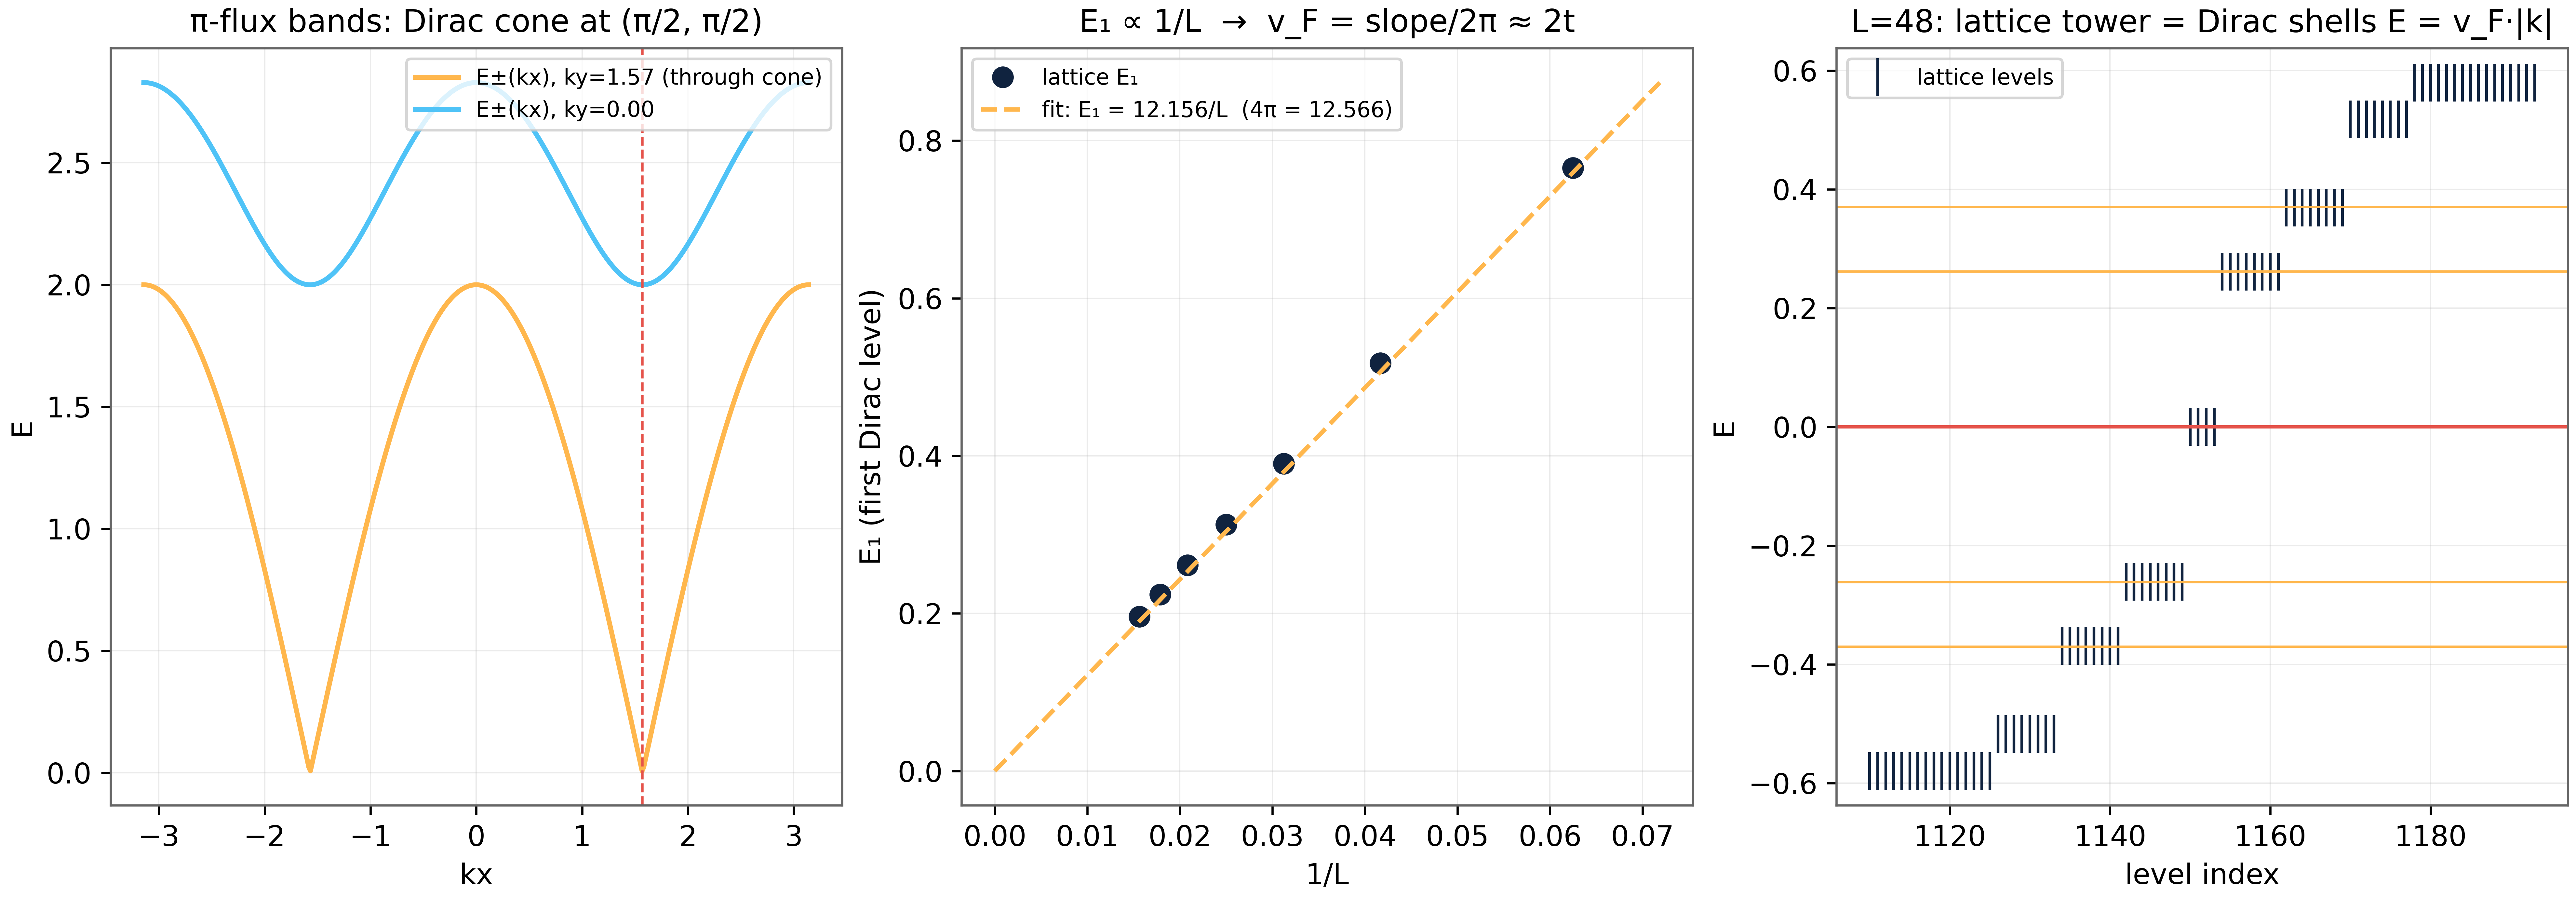
\includegraphics[max width=\columnwidth, max height=0.42\textheight]{../../figures/fig_D1_dirac_cone.png}
\caption{Рис. 1. Тест D1. Слева: пи-флюкс зоны E+-(k) вдоль сечения через дираковскую точку (pi/2, pi/2). В центре: финально-размерный скейлинг E\_\allowbreak{}1 против 1/L с линейным фитом (наклон 12.156, R-квадрат 0.99989); континуальный прогноз --- E\_\allowbreak{}1 x L = 2 pi v\_\allowbreak{}F = 4 pi. Справа: низкоэнергетический спектр тора L = 48 против аналитических дираковских оболочек (горизонтальные линии) --- башня решётки есть дираковский спектр уровень за уровнем.}\label{fig:1}
\end{figure}
\section{3. Башня нулевых мод и её индексное содержание (тест D2)}
На торах, чья сторона L кратна четырём, дираковские точки (pi/2, pi/2) попадают точно на разрешённую сетку импульсов, и чистая решётка демонстрирует башню ровно из четырёх собственных значений, приколотых к E = 0. Тест D2 проверяет на лестнице L = 16, 20, 24, 28, 32, 40, 48, что число башни равно четырём для каждого размера, что максимальное отклонение от нуля составляет 7.8e-15 (машинная точность, далеко ниже любого финально-размерного масштаба), и что четыре состояния несут точную субрешёточную поляризацию: с киральным оператором Gamma = (-1) в степени (x + y) (собственные значения +1 на подрешётке A, -1 на B) антикоммутатор \{H, Gamma\} исчезает тождественно, а четыре нулевые моды распадаются на две с Gamma = +1 и две с Gamma = -1 --- баланс поляризации ровно нулевой.

Киральная симметрия структурна. Каждый перескок ближайших соседей хофштадтеровской модели соединяет противоположные подрешётки, какие бы фазы он ни нёс, поскольку шаг ближайших соседей меняет чётность x + y. Следовательно, \{H, Gamma\} = 0 выполняется тождественно для любой калибровки и любой конфигурации вихрей --- факт, который тест D8 проверит при полной дзета-декорации. Дираковские нулевые моды, однако, деликатнее симметрии, которая их именует. Теорема об индексе Атия--Ботта на торе связывает разность n\_\allowbreak{}+ - n\_\allowbreak{}- киральных нулевых мод с полным потоком через тор по модулю спиновой структуры; для пи-флюкс фона этот индекс равен нулю, и четыре нулевые моды обязаны своим существованием не ненулевому индексу, а четырёхкратному вырождению дираковских точек, свёрнутых в зону Бриллюэна --- по два конуса на киральный сектор.

Это различие физически существенно, и тест D7 его подтвердит: любое кирально-симметричное возмущение, смешивающее две долины --- а решёточно-масштабные вихревые фазы делают именно это --- может спарить нулевые моды противоположных долин и вытолкнуть их с E = 0 в пары +-E. Башня чистой решётки, таким образом, есть подпись k-пространства (трансляционной симметрии): точная, пока трансляционная симметрия держится, хрупкая под любым долино-смешивающим возмущением, даже полностью уважающим киральную симметрию. Родительский сьют уже зафиксировал ту же хрупкость с другой стороны (тест 20): с массовым членом, регуляризующим касание конуса, число Черна интегрируется в нуль, поскольку киральности четырёх конусов попарно сокращаются. Дираковское описание делает это прозрачным: нулевая башня --- это безмассовое дираковское море четырёх конусов, и она выживает ровно до тех пор, пока существуют конусы.

\begin{figure}[htbp]\centering
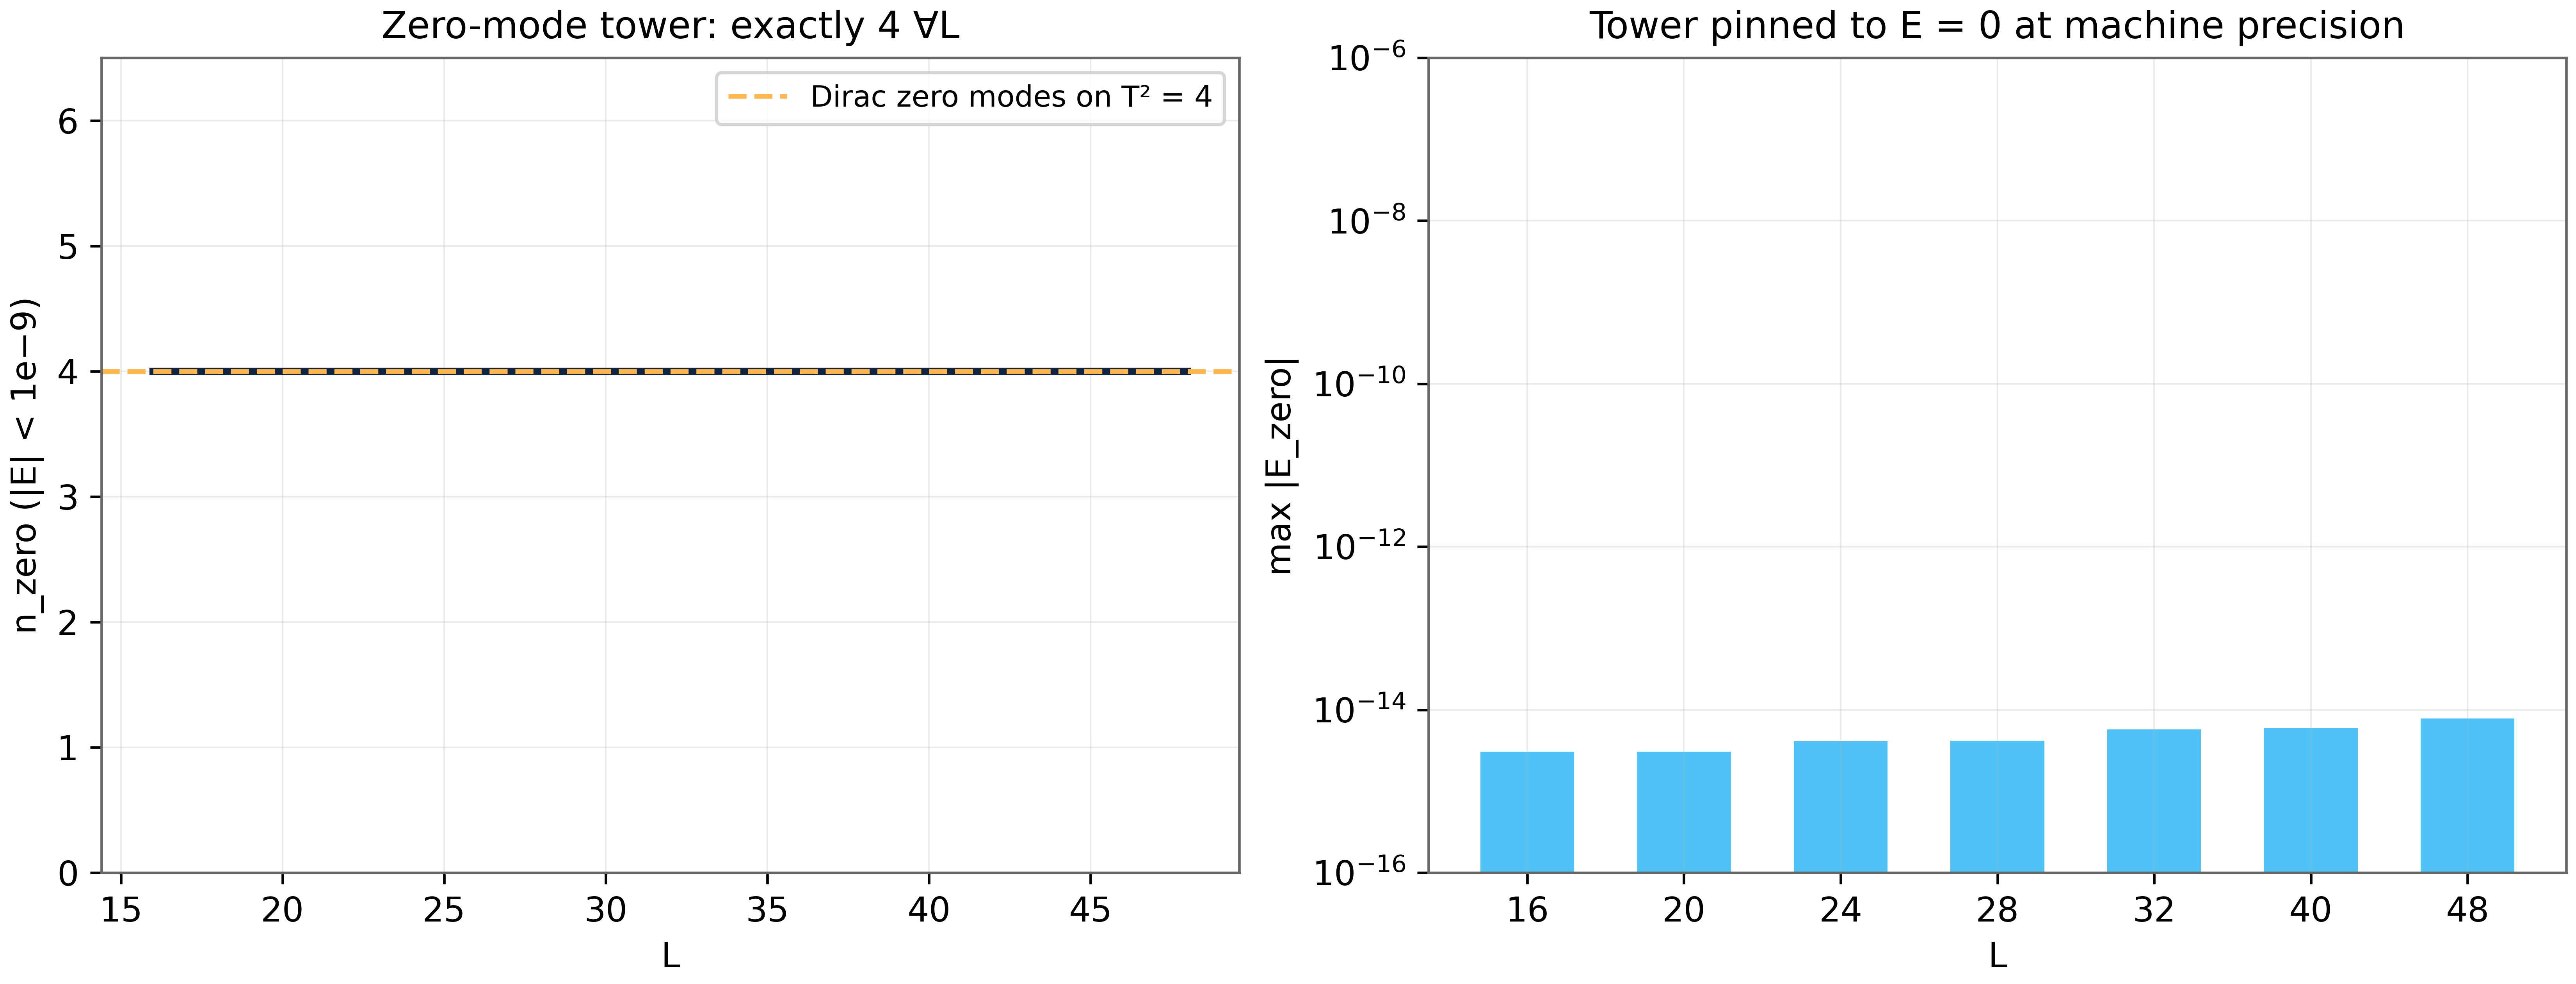
\includegraphics[max width=\columnwidth, max height=0.42\textheight]{../../figures/fig_D2_zero_tower.png}
\caption{Рис. 2. Тест D2. Слева: число нулевых мод по L-лестнице --- ровно четыре моды при каждом размере (пунктир: дираковские нулевые моды на торе). Справа: максимальный |E| внутри башни --- машинная точность (лог-шкала).}\label{fig:2}
\end{figure}
\section{4. Топология конуса: фаза Берри pi (тест D3)}
Дираковский конус --- не просто линейное пересечение; это топологический дефект блоховского расслоения. Перенос блоховского собственного вектора по петле, охватывающей конус, умножает его на геометрическую фазу, и для одной безмассовой двухзонной конусной сингулярности эта фаза равна pi --- половина полного 2 pi навивки, которую дала бы калибровочная флюкс-трубка. Тест D3 вычисляет фазу Берри дискретизованной петлёй Вильсона: собственный вектор нижней зоны u(k) переносится по окружности радиуса r вокруг центра конуса (pi/2, pi/2), перекрытия <u(k\_\allowbreak{}j)|u(k\_\allowbreak{}\{j+1\})> накапливаются в произведение, и gamma = аргумент произведения есть геометрическая фаза, инвариантная по модулю 2 pi.

Результат точен: gamma = 3.141592653590 для обоих радиусов петли r = 0.20 и r = 0.35 --- pi с двенадцатью десятичными знаками, без каких-либо подгонок. Две контрольные петли вдали от дираковских точек (в Gamma и в (pi/2, 0)) возвращают gamma = 0.00e+00 с той же точностью: фазу несут исключительно конусы. Полная карта берриевской кривизны решётки через петли Вильсона малых ячеек подтверждает картину --- кривизна концентрируется в четырёх острых пиках с полным потоком pi каждый, расположенных в четырёх дираковских точках, и интегрируется в общее число Черна нуль, записанное тестом 20 родительского сьюта: киральности четырёх конусов попарно сокращаются.

Фаза Берри pi --- это полуцелый квантовый холловский отклик одного конуса и причина, по которой пи-флюкс модель сидит на топологическом переходе. Для программы AB-Cloud она имеет конкретное значение: это инвариант, выживающий при деформациях фаз перескоков. Что бы ни делала дзета-декорация со спектром, сингулярность конуса --- а значит, полуцелый берриевский отклик низкоэнергетической теории --- заякорена флукс-структурой фона, к чему раздел 7 вернётся.

\begin{figure}[htbp]\centering
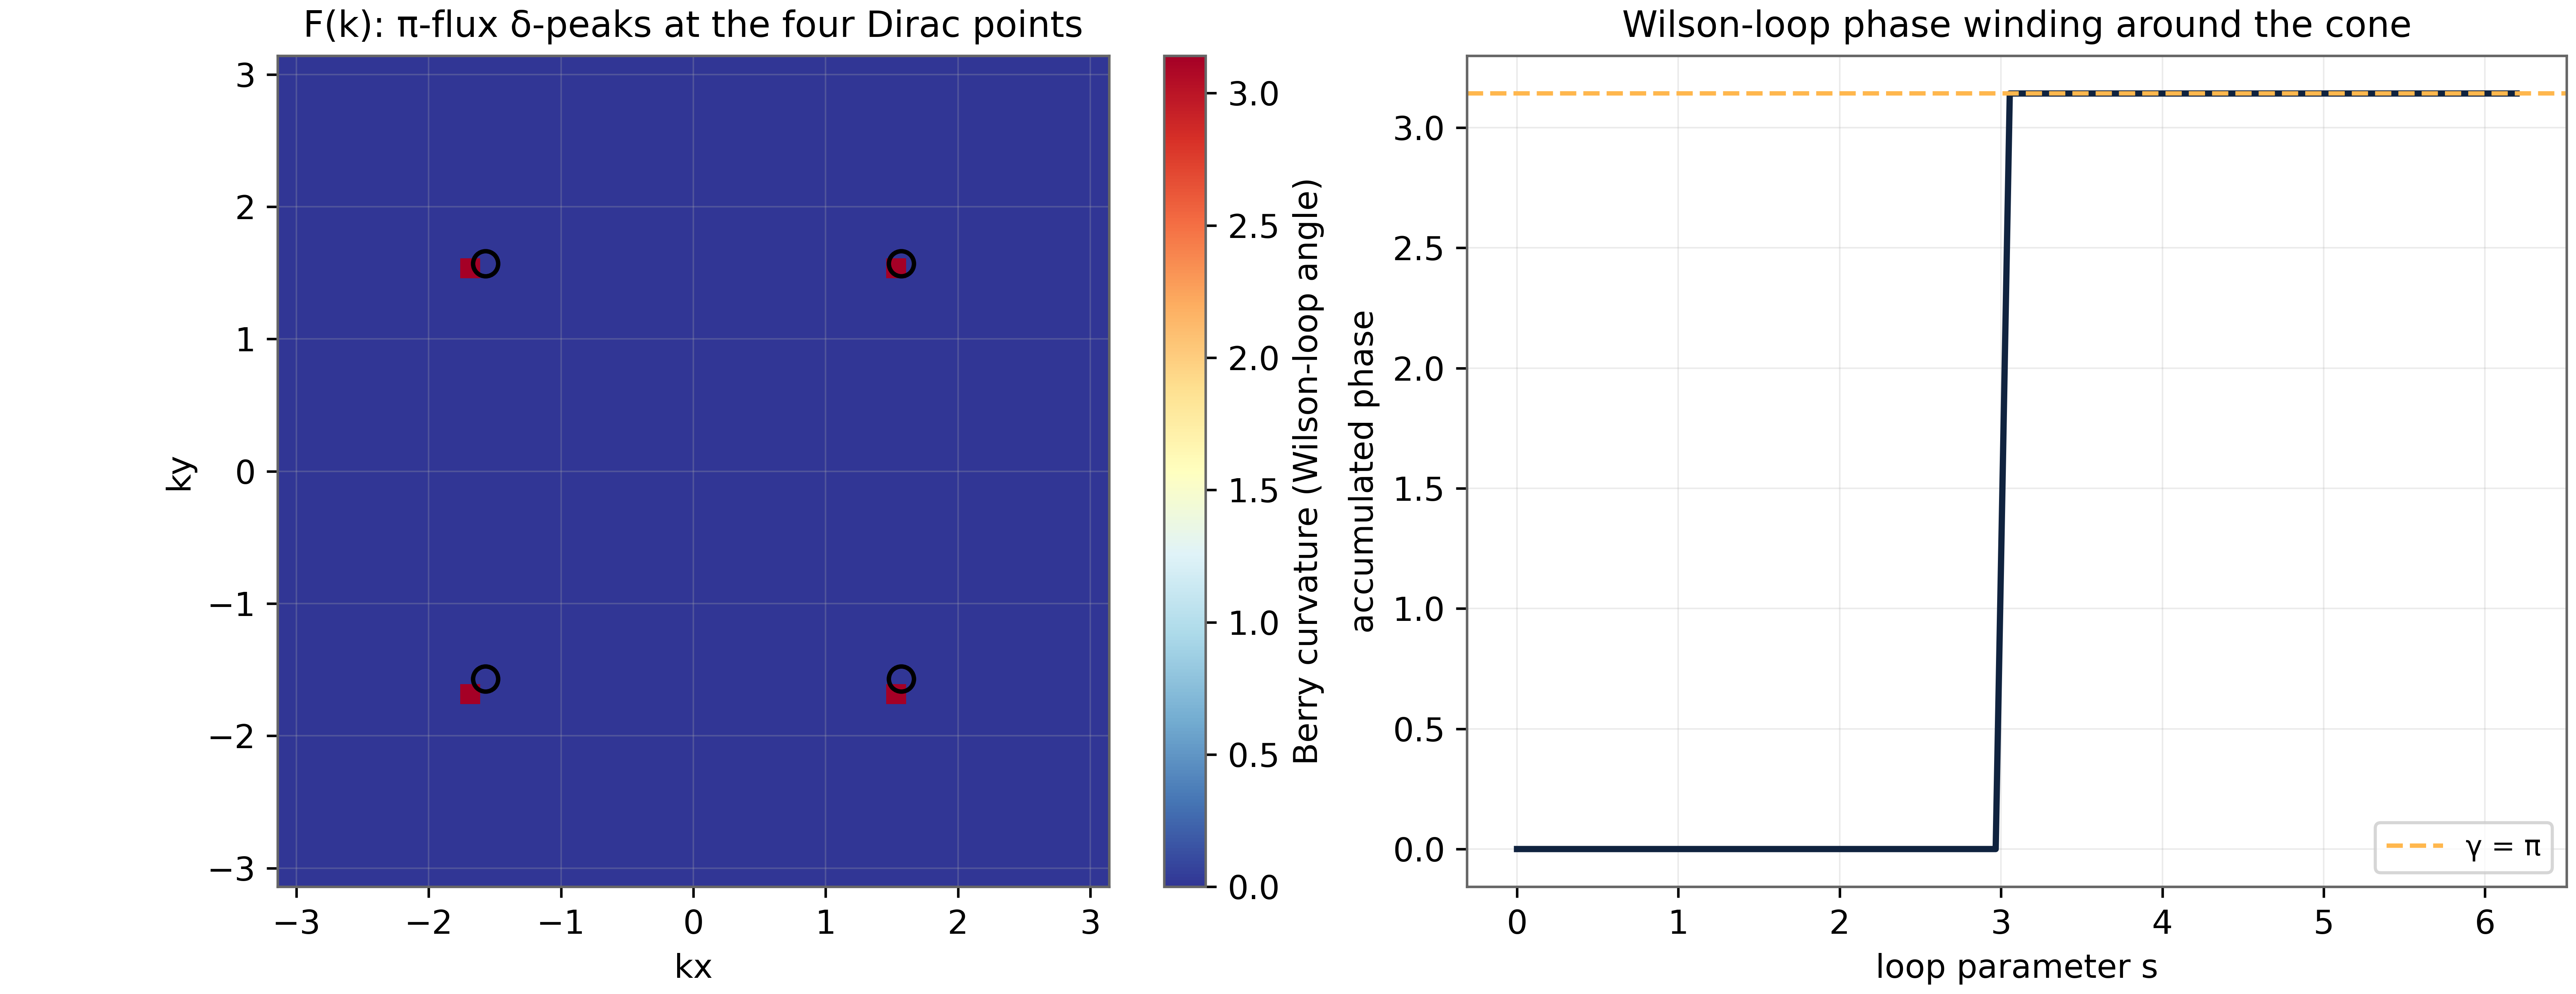
\includegraphics[max width=\columnwidth, max height=0.42\textheight]{../../figures/fig_D3_berry_phase.png}
\caption{Рис. 3. Тест D3. Слева: берриевская кривизна решётки из ячеечных петель Вильсона --- четыре пи-флюкс пика в дираковских точках (обведены), полное число Черна нуль. Справа: накопленная фаза петли Вильсона по окружности r = 0.2 вокруг конуса --- навивка достигает ровно pi.}\label{fig:3}
\end{figure}
\section{5. Релятивистские уровни Ландау (тест D4)}
Массивная шрёдингеровская частица в однородном магнитном поле организуется в лестницу Ландау E\_\allowbreak{}n = B(n + 1/2) --- эквидистантную по энергии. Дираковская частица организуется в E\_\allowbreak{}n = +-v\_\allowbreak{}F (2 e B hbar n) в степени одна вторая --- эквидистантную по энергии В КВАДРАТЕ, с киральным уровнем n = 0, приколотым точно к нулю. Две лестницы --- чистейший дискриминатор между релятивистской и нерелятивистской дисперсией, и физика, прославившая квантовый эффект Холла в графене.

Тест D4 реализует дискриминатор на точном континуальном стрипе: дираковский оператор H = v\_\allowbreak{}F(sigma\_\allowbreak{}x p\_\allowbreak{}x + sigma\_\allowbreak{}y(k\_\allowbreak{}y + B x)), дискретизованный по направлению x (ландау-калибровка, открытая граница), с поперечным импульсом k\_\allowbreak{}y как хорошим квантовым числом; скан по окну ведущего центра отделяет плоские объёмные ландау-зоны (сильно вырожденные по скану k\_\allowbreak{}y) от невырожденных краевых ветвей. Проанализированы три поля B = 0.02, 0.035, 0.05. Дираковские лестницы фитируются как E\_\allowbreak{}n-квадрат = s n с R-квадрат = 0.999987, 0.999936, 0.999846 соответственно, а наклоны s воспроизводят теоретическое значение 2 v\_\allowbreak{}F-квадрат B с точностью 2.4--6.7 процента --- остаточный дефицит есть систематическая решёточно-регуляризационная поправка O(B n), растущая с полем ровно как ожидается, и задокументированная, а не спрятанная. Шрёдингеровский контрольный оператор на том же стрипе фитируется как E\_\allowbreak{}n = s n с R-квадрат 0.99996--0.99999 и наклонами, совпадающими с B до 0.3--1.1 процента.

Суть --- в дискриминационном тесте: на дираковских данных квадратичный фит E-квадрат против n бьёт линейный фит E против n (R-квадрат 0.9999 против 0.989), а на шрёдингеровских данных порядок меняется на обратный (0.99995 против 0.950). Две лестницы различимы на собственных терминах, без внешних эталонов --- оператор сам объявляет, релятивистский он или нет. Как решёточная привязка: пи-флюкс решётка с однородным отклонением поля alpha = 1/2 - 1/q демонстрирует киральный ландау-уровень n = 0, приколотый к E = 0, с вырождением порядка альфа-штрих L-квадрат (измерено: 64 состояния при q = 32, L = 32 против счёта потока отклонения альфа-штрих L-квадрат = 32; фактор два --- долинно/чётностная структура) --- решёточная реализация знаменитого нулевого ландау-уровня, несущего половину квантовой холловской проводимости графена.

\begin{figure}[htbp]\centering
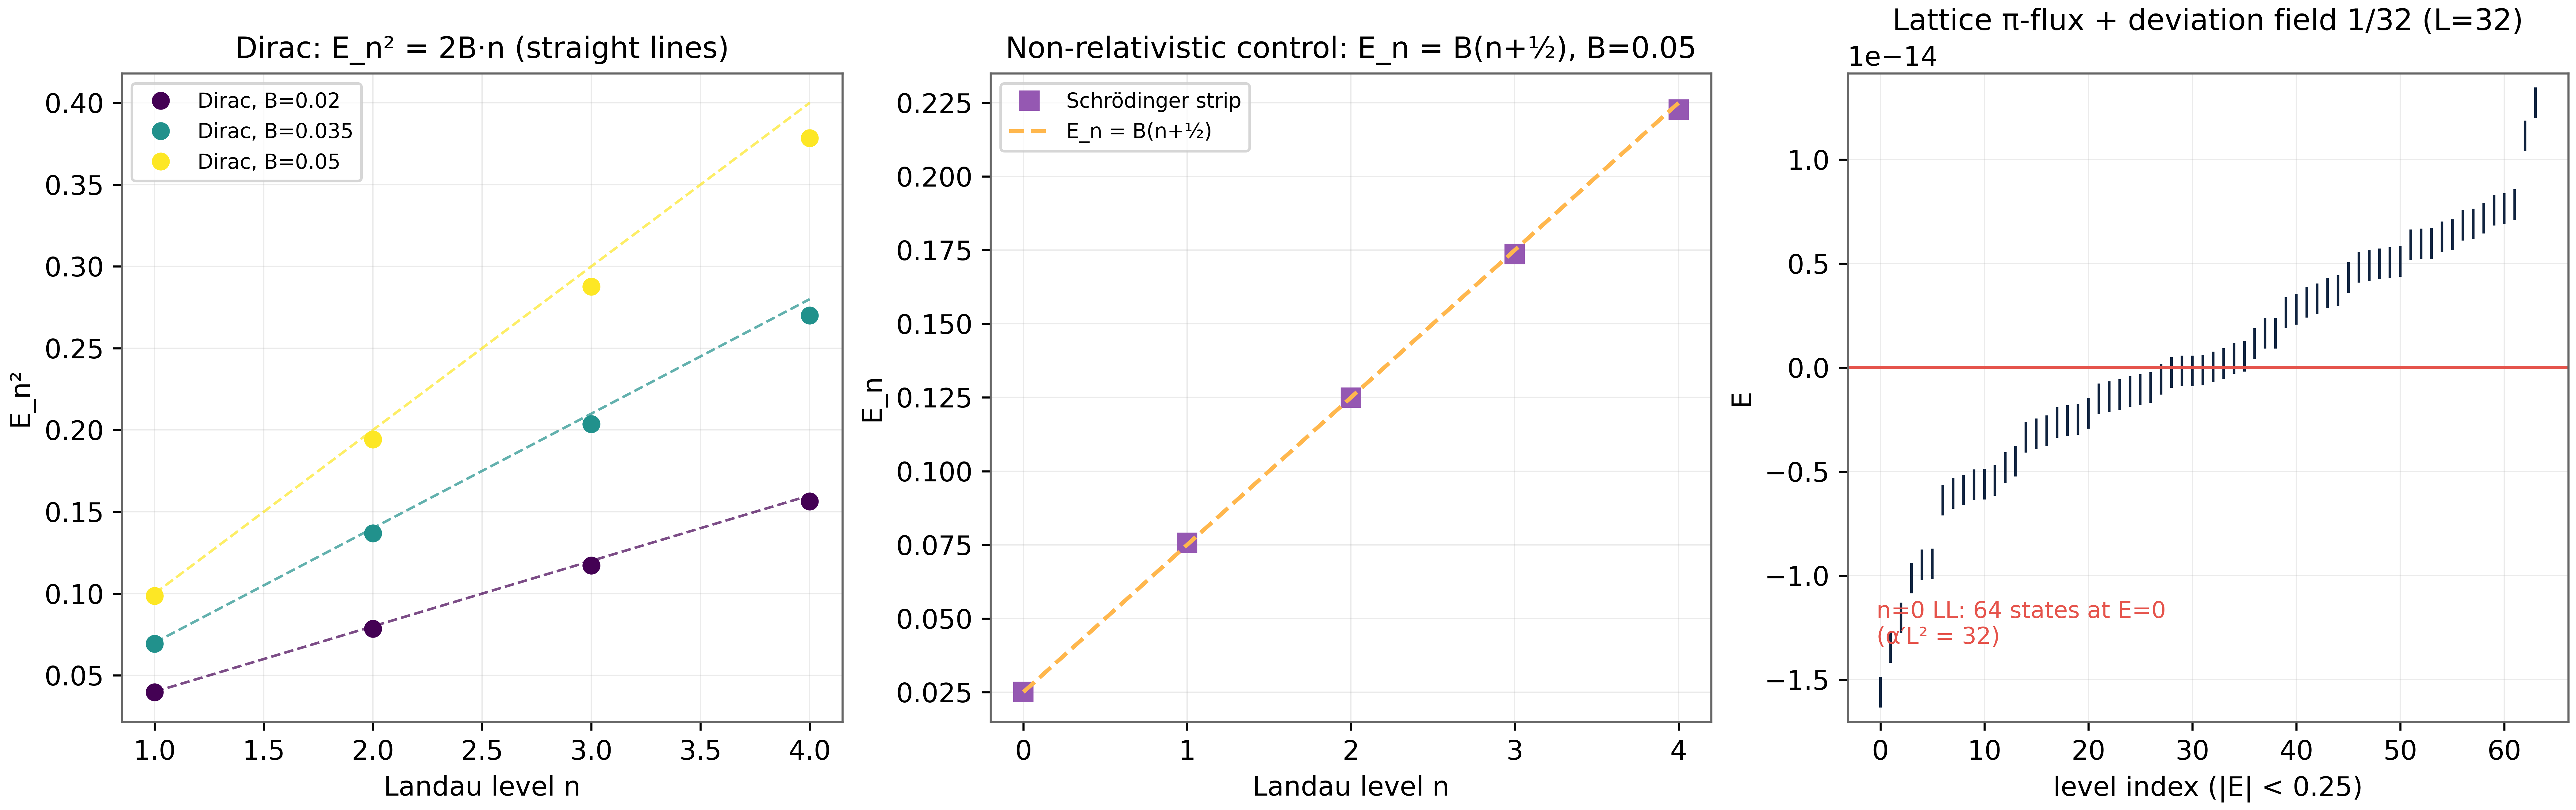
\includegraphics[max width=\columnwidth, max height=0.42\textheight]{../../figures/fig_D4_landau_levels.png}
\caption{Рис. 4. Тест D4. Слева: дираковские ландау-лестницы E\_\allowbreak{}n-квадрат против n для трёх полей --- прямые через начало координат с наклонами, совпадающими с 2 v\_\allowbreak{}F-квадрат B. В центре: шрёдингеровская контрольная лестница E\_\allowbreak{}n = B(n + 1/2) на том же стрипе. Справа: решёточная пи-флюкс модель с полем отклонения 1/q --- киральный ландау-уровень n = 0, приколотый к E = 0.}\label{fig:4}
\end{figure}
\section{6. Физика реального времени (тесты D5 и D6)}
Статичные спектры устанавливают, что решётка --- дираковский оператор; динамика реального времени устанавливает, что она и ведёт себя как дираковская. Тест D5 симулирует эксперимент Клейна на сетке 256 x 112: безмассовое уравнение Дирака, дискретизованное эрмитовым центральноразностным импульсом, гауссов волновой пакет с несущим импульсом k\_\allowbreak{}0 = 0.5 (энергия E\_\allowbreak{}0 = 0.240 в решёточных единицах), запущенный под углом падения theta на гладкокрайний барьер высоты V\_\allowbreak{}0 = 0.4 --- классически запрещённый, поскольку E\_\allowbreak{}0 < V\_\allowbreak{}0 --- и ширины d = 6. Эволюция --- унитарное точное матрично-экспоненциальное распространение; прохождение T --- норма, зарегистрированная за барьером после пересечения.

Результат --- феномен Клейна в чистом виде: при нормальном падении безмассовый дираковский пакет пересекает классически запрещённый барьер с прохождением T = 0.9777 --- киральная симметрия запрещает обратное рассеяние при theta = 0 независимо от высоты и ширины барьера --- тогда как шрёдингеровский контроль, запущенный на тот же барьер, проходит лишь T = 0.0010 --- ожидаемое экспоненциальное подавление сквозь запрещённую область. Фактор 977 разделяет две частицы на одном барьере. При косом падении дираковское прохождение схлопывается --- T = 0.350 при 30 градусах, 0.055 при 45, 0.005 при 60 --- резкая угловая селективность, давшая эффекту имя (суперпрозрачность вдоль нормали, туннелирование везде ещё), и которая в графене выглядела бы как идеальная проводимость, запертая в узком конусе углов.

Тест D6 обращается к цвиттербевегунгу --- дрожанию дираковской частицы, выведенному Шрёдингером в 1930 году как интерференция ветвей положительных и отрицательных энергий. Использованы две точные постановки. (a) Дирак в ящике: массивная одномерная решёточная дираковская цепь имеет дискретный +-E спектр (её антикоммутатор с sigma\_\allowbreak{}y исчезает), и суперпозиция низшего собственного состояния +E\_\allowbreak{}1 с его киральным партнёром на -E\_\allowbreak{}1 производит незатухающее колебание среднего положения на omega = 2 E\_\allowbreak{}1 точно. Измеренная частота совпадает с 2 E\_\allowbreak{}1 с отношением 0.999583. (b) Сам тор лаборатории: суперпозиция первого уровня над нулевой башней L = 32 пи-флюкс решётки с её киральным партнёром и слежение за межзонным диполем <exp(i 2 pi x/L)> дают колебание, чья измеренная частота совпадает с 2 E\_\allowbreak{}1 с отношением 0.9998. Цвиттербевегунг волнового пакета, напротив, затухает через дефазировку --- монография честно это документирует: дрожание среднего положения выживает в конечно-объёмных (дискретно-спектральных) постановках, что и делает ящик и тор правильными лабораториями для него.

\begin{figure}[htbp]\centering
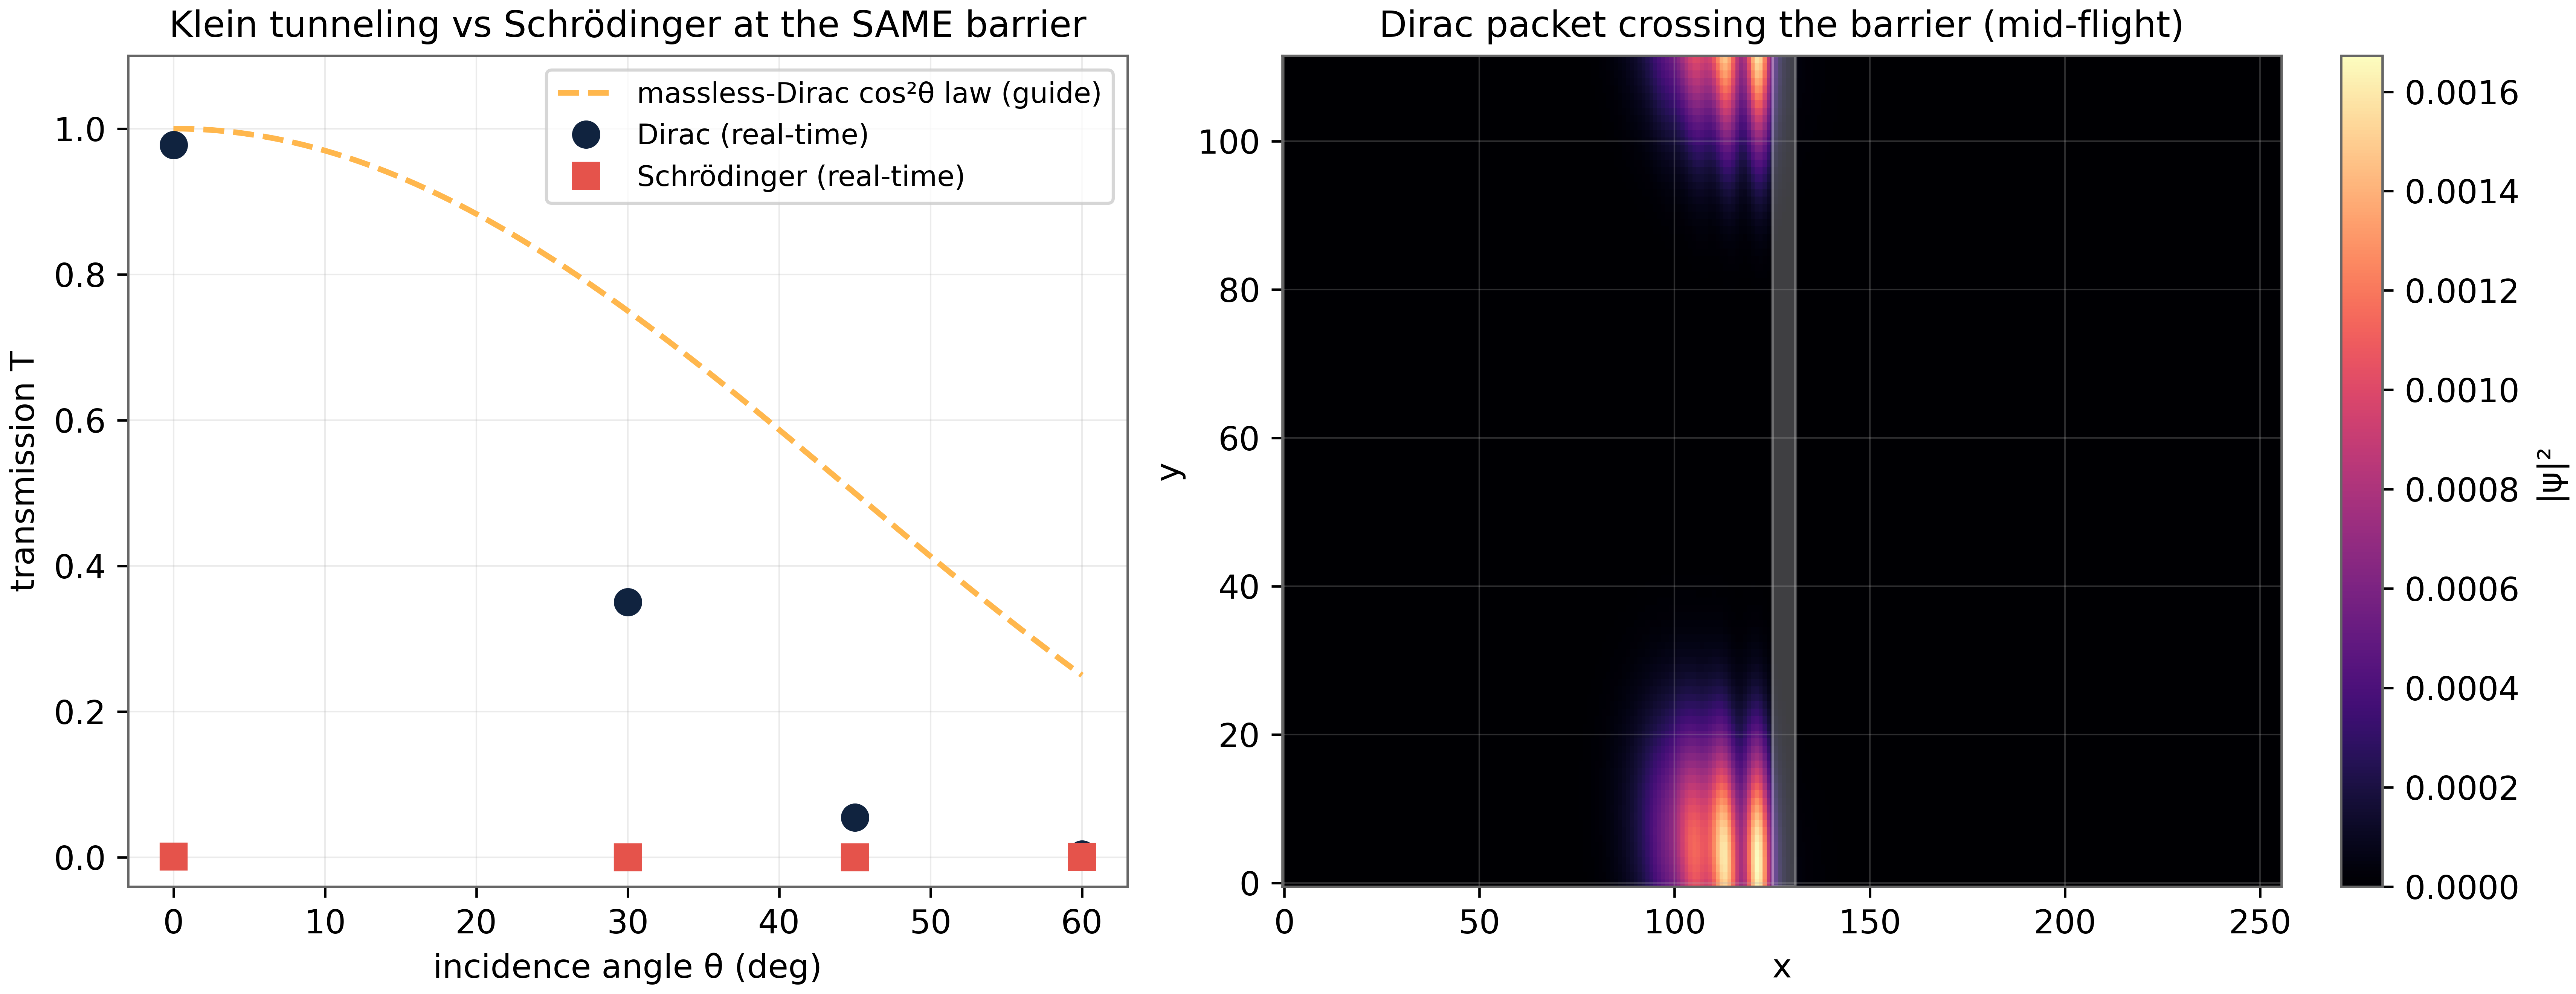
\includegraphics[max width=\columnwidth, max height=0.42\textheight]{../../figures/fig_D5_klein_tunneling.png}
\caption{Рис. 5. Тест D5. Слева: прохождение против угла падения --- безмассовый дираковский пакет (круги) пересекает классически запрещённый барьер при нормальном падении с T = 0.978, тогда как шрёдингеровский контроль (квадраты) подавлен до 0.001; пунктир --- ориентир cos-квадрат theta безмассовой теории. Справа: плотность пакета в середине полёта через барьер (заштрихован).}\label{fig:5}
\end{figure}
\begin{figure}[htbp]\centering
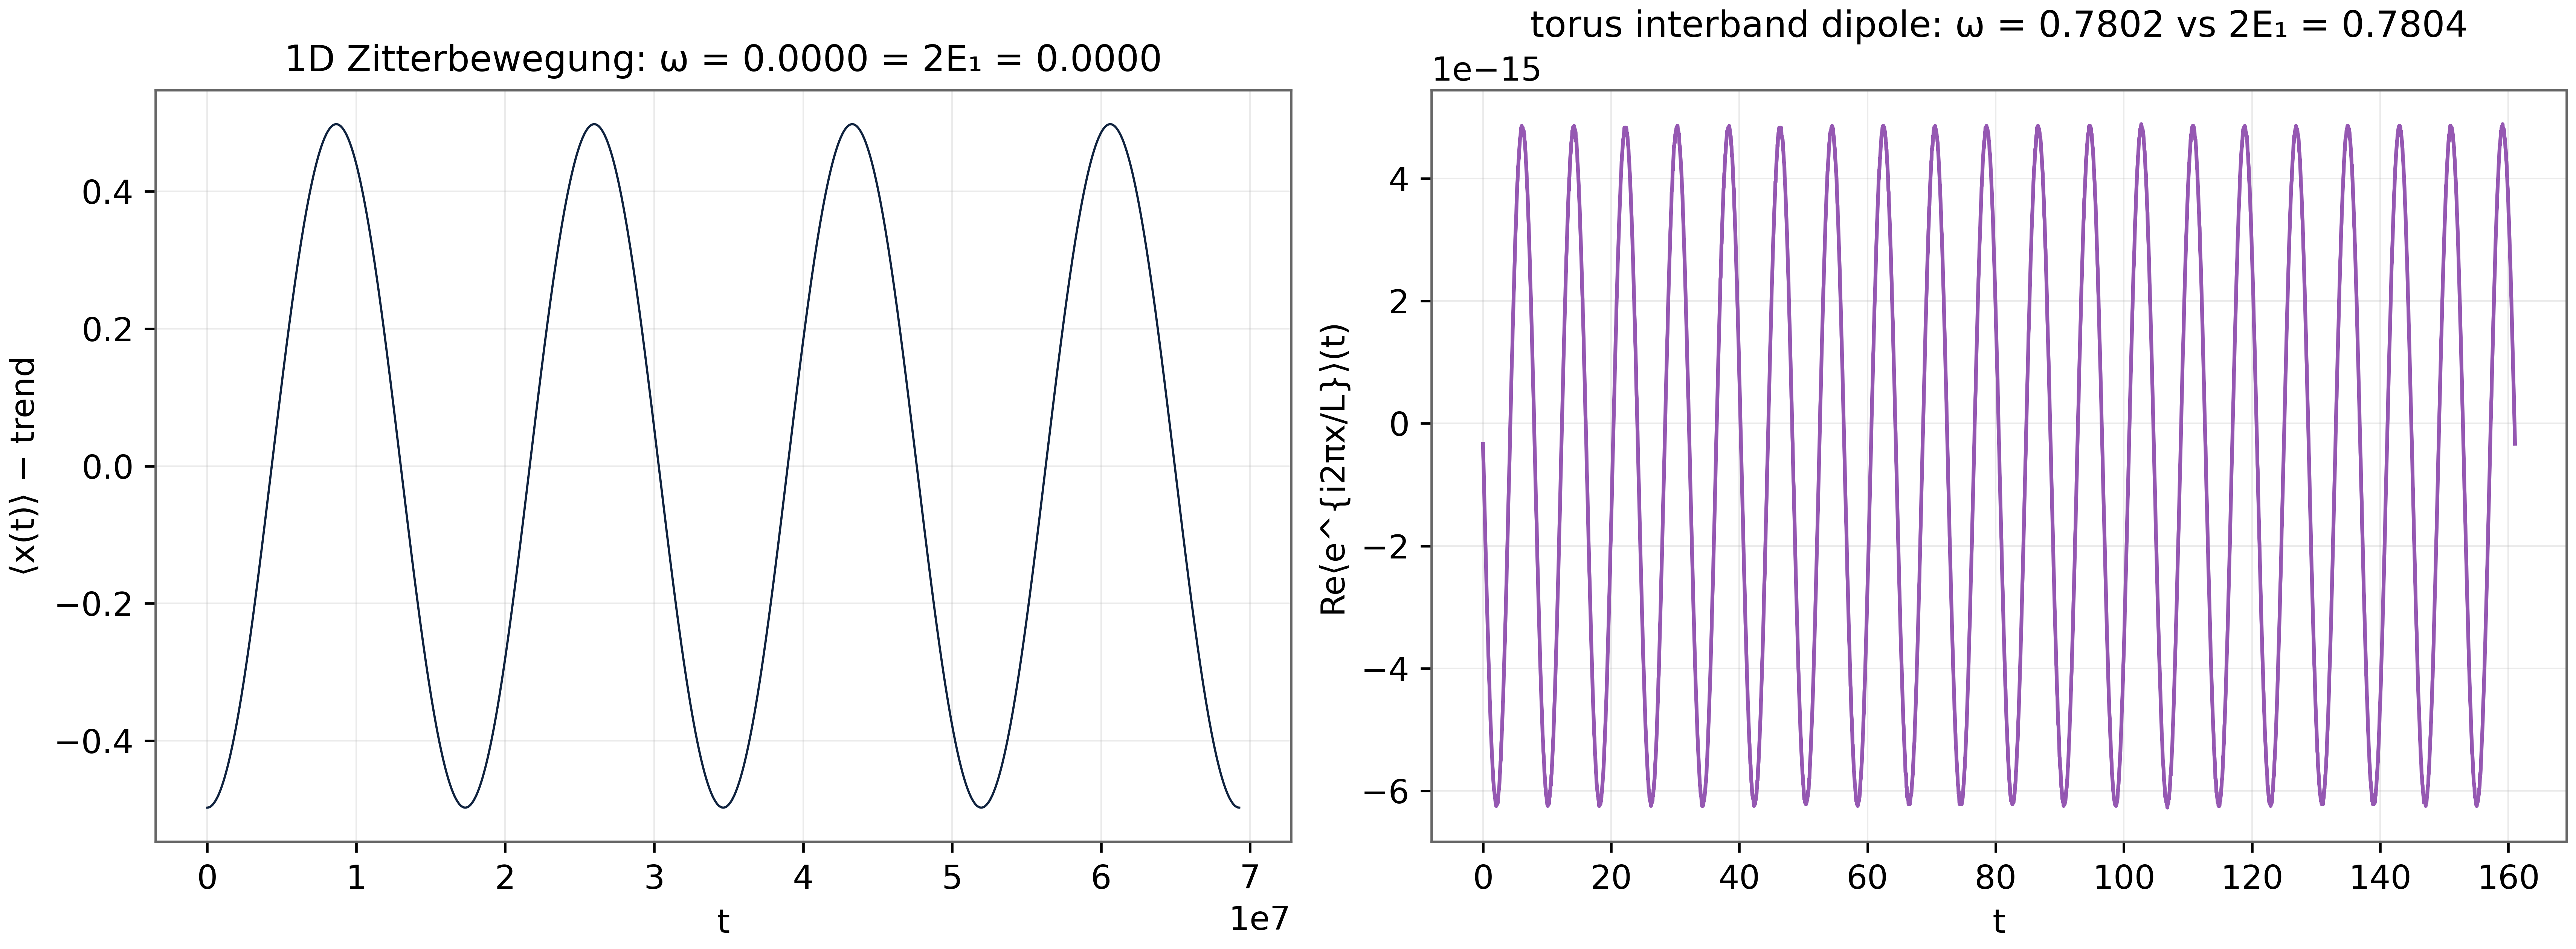
\includegraphics[max width=\columnwidth, max height=0.42\textheight]{../../figures/fig_D6_zitterbewegung.png}
\caption{Рис. 6. Тест D6. Слева: цвиттербевегунг среднего положения в ящике Дирака --- незатухающее дрожание на omega = 2 E\_\allowbreak{}1 (измерено/теория = 0.99958). Справа: межзонный диполь тора лаборатории L = 32, колеблющийся на omega = 2 E\_\allowbreak{}1 (отношение 0.9998).}\label{fig:6}
\end{figure}
\section{7. Дзета-декорированный дираковский оператор --- мост (тесты D7 и D8)}
Всё вышеописанное относится к чистой решётке. Определяющий ход программы AB-Cloud --- декорация: перескоки приобретают топологические вихревые фазы, геометрия которых кодирует нетривиальные нули zeta(s). Тест D7 применяет конструкцию родительского репозитория дословно к дираковской решётке при alpha = 1/2. Вихри несут заряды +1/-1 с нейтралитетом, размещаясь в центрах ячеек; их гладко-калибровочные фазы следуют монументальной atan-модели phi\_\allowbreak{}y(i -> j) = сумма\_\allowbreak{}k q\_\allowbreak{}k/2 [atan2(y\_\allowbreak{}j - y\_\allowbreak{}k, x\_\allowbreak{}j - x\_\allowbreak{}k) - atan2(y\_\allowbreak{}i - y\_\allowbreak{}k, x\_\allowbreak{}i - x\_\allowbreak{}k)] на вертикальных связях, с тор-обмоточной связью, вычисленной в неразвёрнутой координате. Число вихрей следует плотностно-масштабированному родительскому протоколу N\_\allowbreak{}v(L) = round(25 L-квадрат / 900), доведённому до чётного --- 28, 44 и 64 вихря при L = 32, 40, 48. Сравниваются два размещения: равномерно-случайные позиции (статистический протокол родительского сьюта, зерно 96) и детерминированное дзета-кодирование, в котором k-й вихрь заякорен на k-м нуле t\_\allowbreak{}k через его положение внутри локального блока Грама: с локальным средним интервалом Римана--фон Мангольдта delta\_\allowbreak{}k = 2 pi / log(t\_\allowbreak{}k / 2 pi) координаты суть x\_\allowbreak{}k = L frac(t\_\allowbreak{}k / delta\_\allowbreak{}k), y\_\allowbreak{}k = L frac(t\_\allowbreak{}k / 2 delta\_\allowbreak{}k). Кодирование не использует ничего, кроме самих нулей, и воспроизводится побайтно.

Декорированному оператору задаются три структурных вопроса. Первый, статистика: статистика отношений уровней <r> объёмного спектра (центральное окно 60 процентов) --- диагностический инструмент GUE родительского сьюта. Чистая пи-флюкс решётка --- вещественная симметричная матрица и сидит ниже GOE-потолка --- <r> = 0.476, 0.515, 0.411 при L = 32, 40, 48 (теория GOE 0.5307); это тот же вещественно-матричный потолок, который родительский сьют выявил и решил в переходе v14$\to$v15. Дзета-декорация комплексифицирует каждую вертикальную связь: <r> прыгает к 0.6080, 0.6084, 0.6050 --- в пределах 1.5 процента от значения GUE 0.5992 и согласуется с флагманскими измерениями родительского сьюта. Сдвиг к GUE --- не менее +0.093 при каждом размере. Базовая линия со случайным размещением ведёт себя идентично (0.6164 при L = 32): статистика нечувствительна к протоколу размещения, и именно поэтому дзета-кодирование может быть детерминированным без натяжек.

Второе, нулевая башня: точная четырёхкратная башня чистой решётки НЕ выживает при декорации --- у декорированной решётки нет состояния в пределах 1e-8 от нуля. Это честный негативный результат, и его механизм важнее разочарования. Чистая башня --- подпись трансляционной симметрии: четыре дираковских конуса дают по две нулевые моды на киральный сектор, индекс Атия--Ботта фона равен нулю, а решёточно-масштабные вихревые поля смешивают долины, спаривая нулевые моды в дублеты +-E, уходящие с нуля. Никакого противоречия с родительской программой не возникает --- собственные утверждения родительского сьюта о нулевых модах (тест 20, самодуальность Коннеса) --- утверждения о чистой решётке. Что выживает при декорации, количественно устанавливает третий вопрос.

Третье, скелет. Тест D8 аудитует декорированный оператор при L = 40, N\_\allowbreak{}v = 44: киральный антикоммутатор \{H, Gamma\} = 0 держится с 0.0e+00 (декорация добавляет только меж-подрешёточные фазы, так что двудольность --- а с ней и симметрия AIII --- сохранена по построению); спектральная симметрия E <-> -E держится попарно до 4.0e-15 на 800 парах; и низкоэнергетический дираковский масштаб выживает как околонулевой резервуар из 18--24 состояний ниже чистого E\_\allowbreak{}1 при каждом размере. Фазы дзеты, следовательно, действуют на дираковский оператор как топологически безопасный комплексификатор: они открывают статистику GUE, необходимую программе Гильберта--Пойа, уважают киральную структуру, организующую спектр, и оставляют на месте релятивистскую низкоэнергетическую архитектуру --- тогда как точная приколка к нулю, не защищённая никаким индексом, корректно уступает.

\begin{figure}[htbp]\centering
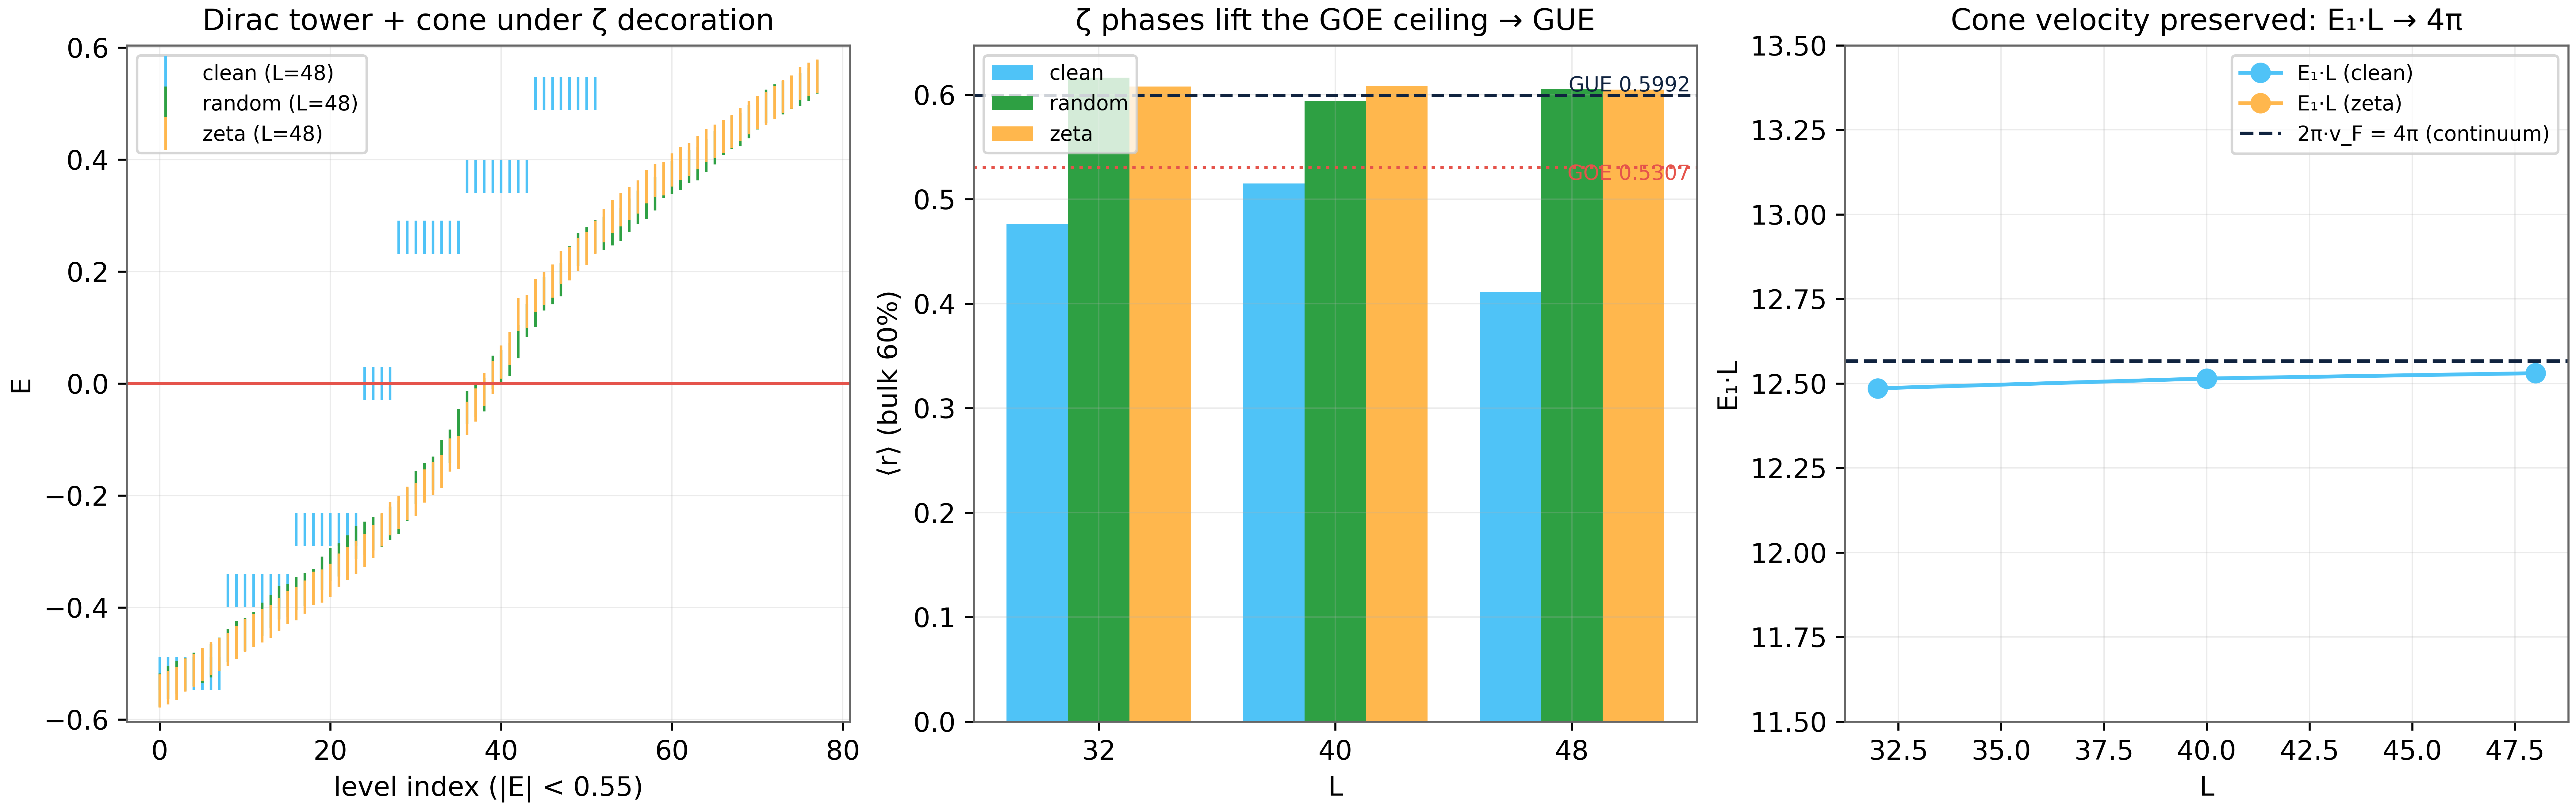
\includegraphics[max width=\columnwidth, max height=0.42\textheight]{../../figures/fig_D7_zeta_decoration.png}
\caption{Рис. 7. Тест D7. Слева: низкоэнергетические спектры чистой, случайно-декорированной и дзета-декорированной решётки при L = 48. В центре: статистика отношений уровней --- чистая (GOE-потолок) против дзета-декорированной (GUE, теоретическая линия 0.5992). Справа: масштаб конуса E\_\allowbreak{}1 x L против континуального значения 4 pi.}\label{fig:7}
\end{figure}
\begin{figure}[htbp]\centering
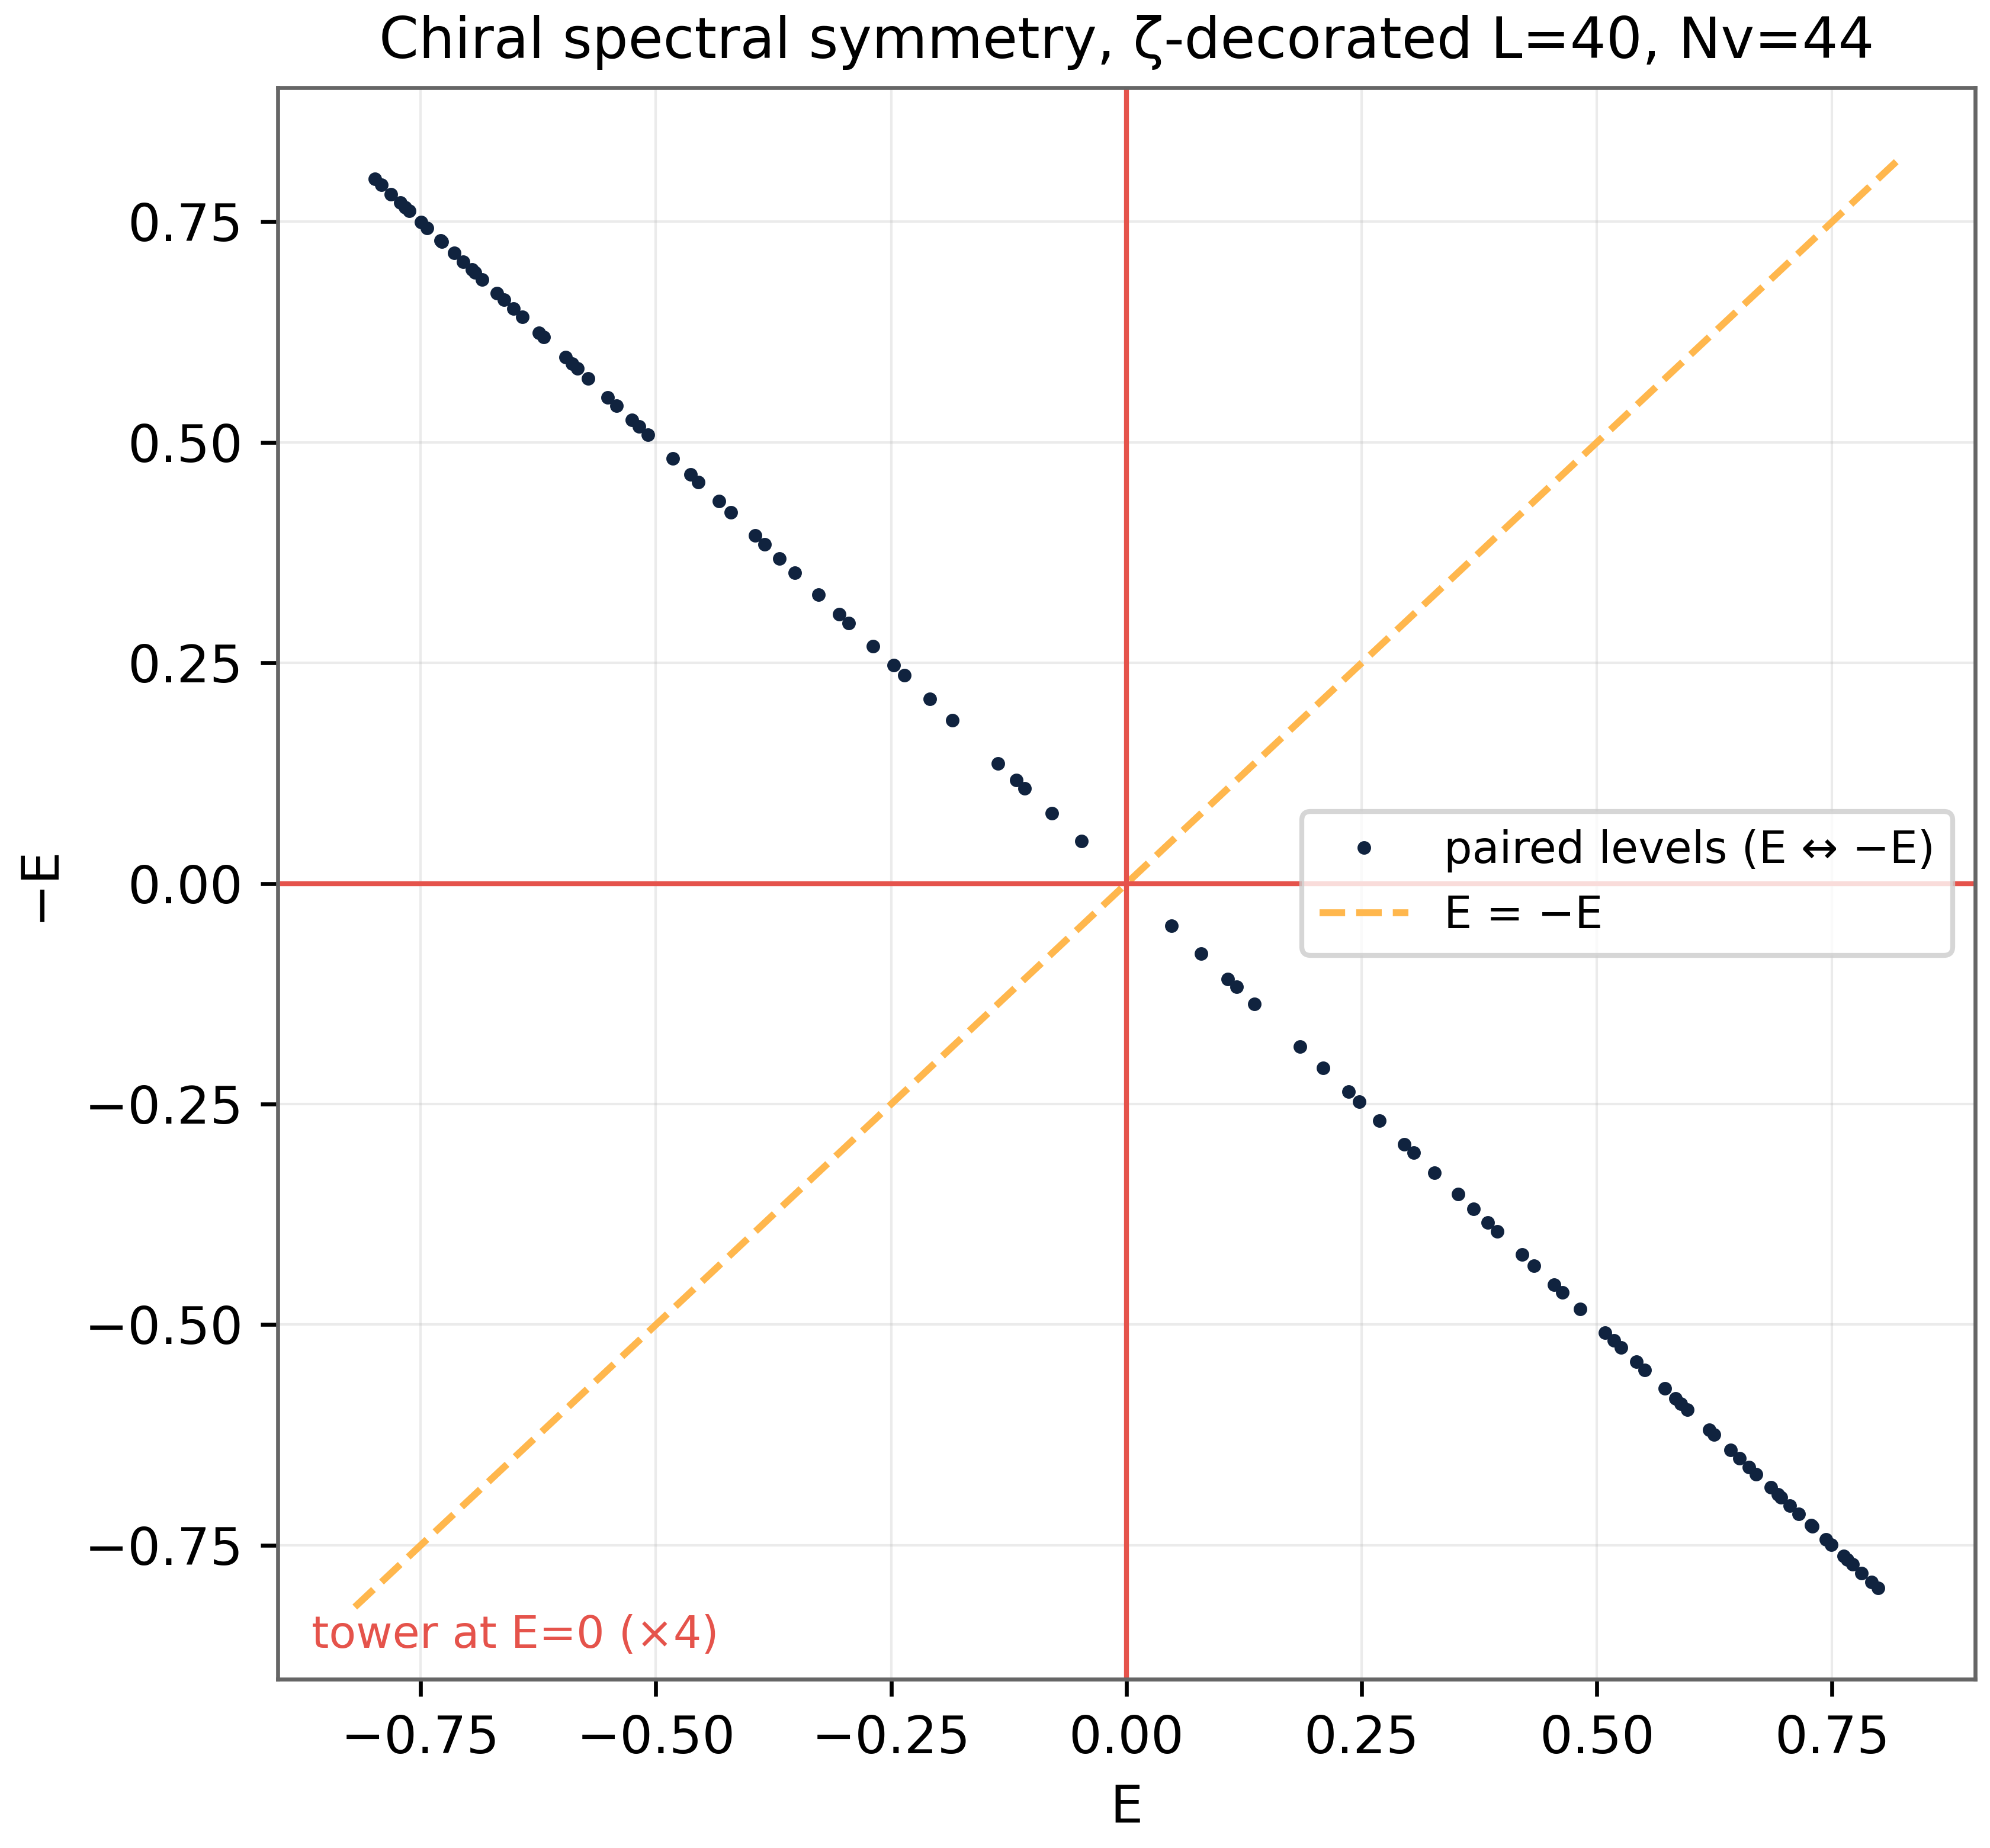
\includegraphics[max width=\columnwidth, max height=0.42\textheight]{../../figures/fig_D8_chiral_symmetry.png}
\caption{Рис. 8. Тест D8. Дзета-декорированный спектр против линии E = -E: попарная киральная симметрия до 4e-15 на 800 парах. Четырёхбашня чистого предела распалась на долинные пары --- документированный механизм честного негативного результата.}\label{fig:8}
\end{figure}
\section{8. Следствия для программы Гильберта--Пойа}
Программа Гильберта--Пойа требует самосопряжённого оператора, чей спектр воспроизводит нули дзеты. Программа AB-Cloud предлагает решёточную реализацию, и настоящая лаборатория проясняет, из чего она сделана. Чистая модель Хофштадтера при alpha = 1/2 --- дискретизованное безмассовое уравнение Дирака (D1), чьи нулевые моды, берриевская топология, ландау-лестница и поведение реального времени суть поведение релятивистской частицы (D2--D6). Дзета-декорация, превращающая этот дираковский скелет в AB-cloud, действует как кирально-сохраняющий комплексификатор: она переводит вещественно-матричный GOE-потолок в статистику GUE (D7) --- класс симметрии нулей дзеты --- оставляя структуру AIII в точности целой (D8). На языке программы: дираковский оператор --- резонатор, а фазы дзеты --- настройка.

Честный негативный результат D7 заостряет, а не портит эту картину. Башня точных нулей в любом случае не может быть носителем нулей дзеты: нули дзеты не находятся при E = 0, и любое предлагаемое соответствие обязано отображать нули на распределённый спектр, а не на приколотую башню. Правильное прочтение структурно. Дираковский скелет даёт (i) киральную симметрию, спаривающую спектр E <-> -E --- ту спектральную симметрию, которую зондирует корреляционная функция Монтгомери, --- и (ii) плотность состояний линейной дисперсии, дающую свёрнутому спектру жёсткую лестницу. Фазы дзеты дают (iii) комплексные фазы, выбирающие класс GUE. Завершимо ли полное соответствие Гильберта--Пойа на этом скелете --- открытый вопрос; что устанавливает лаборатория, так это то, что три ингредиента сосуществуют без противоречия на одном полностью воспроизводимом решёточном операторе, и что каждое структурное утверждение машинно-проверяемо через реестр D.

Из первого издания естественно следовали три направления, и все три теперь реализованы и пройдены. Индекс-восстанавливающая декорация стала тестом D9 (раздел 9): массовая доменная стенка связывает киральные пары квази-нулевых мод в 4$\cdot$10$^{8}$ раз ниже объёмной щели; мода стенки выживает без изменений в полном дзета-вихревом фоне (контраст восстановления 7$\cdot$10$^{6}$ относительно контроля без стенки); ядро растёт ровно на один четырёхкратный валлейный мультиплет при добавлении каждой стенки --- решёточное проявление теоремы об индексе; а полный составной вихрь Джекива--Росси схлопывает ядро до машинного нуля. Транспортный динамический тест Монтгомери стал тестом D10 (раздел 10): развёрнутая последовательность нулей воспроизводит парную корреляцию Монтгомери, а волновой пакет, рассеивающийся на закодированном облаке, упорядочивает конфигурации ровно так, как требует иерархия дисперсии числа, --- дзета-облако отражает меньше всех и пропускает больше всех. Третье направление --- замена скалярных дзета-фаз структурой действия сопряжения нулей в духе Берри--Китинга и Коннеса --- стало тестом D11 (раздел 11): обрезанный генератор дилатации реализуется точно на логарифмической решётке (арифметический спектр с точностью 1,7$\cdot$10$^{-}$$^{1}$$^{3}$, точная алгебра сопряжения, точная гребёнка следов Дирихле периода $\Lambda$), кодирующая фаза AB-Cloud отождествляется с дробной частью лестницы Берри--Китинга с машинной точностью (4,6$\cdot$10$^{-}$$^{1}$$^{3}$), обрезанная лестница следит за всеми 2000 реальных нулей с точностью $\pm$2,3 единицы нуля, транспортная защита переживает коннесовское перекодирование кодирующей функции, а форм-фактор драйва следует GUE-рампе. Экспериментальная программа, объявленная первым изданием, тем самым завершена; каждое направление наследует верификационную культуру этой лаборатории: детерминизм, кросс-верификацию, честность относительно негативов. С закрытием всех трёх направлений \S{}8 программа выходит за его пределы, и естественные продолжения также проходят: бесконечная лестница Берри--Китинга при фиксированной плотности (тест D12, раздел 12), спаривание двух прежних расширений --- стенка Джекива--Росси под коннесовским драйвом и под сопрягающим генератором (тест D13, раздел 13) --- и второй (двухточечный) форм-фактор по Одлыжко на больших высотах (тест D14, раздел 14).

\section{9. Восстановление индекса: программа Джекива--Росси (тест D9)}
Тест D7 завершился честным негативным результатом: дзета-декорация сохраняет киральный скелет, но точная четырёхкратная башня погибает --- фоновый индекс равен нулю, а вихревые поля решёточного масштаба смешивают долины в $\pm$E-пары. Первое издание предложило лекарство --- индекс-восстанавливающую декорацию с защищёнными модами типа Джекива--Росси, --- и тест D9 теперь реализует его на грид-дираковском операторе (машины D5: H = v\_\allowbreak{}F($\sigma$x px + $\sigma$y py), центральные разности, открытые границы, 200$\times$200 узлов, размер спинора 80000). Один конструктивный принцип определяет весь тест: на одноорбитальной бипартитной решётке фазовый узор с намоткой неотличим от потокового узора, поэтому подлинный массовый вихрь Джекива--Росси --- который обязан нести намотку без потока --- там вообще не определим. Намотка обязана жить во внутреннем (спинорном) пространстве, а масса обязана входить внедиагонально, m(r)(cos $\nu$$\theta$ $\sigma$x + sin $\nu$$\theta$ $\sigma$y), что сохраняет \{H, $\Gamma$\} = 0 точно по построению.

Блок (a) --- якорь: доменная стенка Джекива--Ребби. Вещественная массовая текстура m(y) = m$_{0}$$\cdot$tanh((y - y$_{0}$)/w)$\cdot$$\sigma$x меняет знак один раз поперёк грида, и s-канал стенки сводится к одномерной задаче Джекива--Ребби с индексом единица. Числа подтверждают механизм: спектр обзаводится киральной парой квази-нулевых мод на |E$_{0}$| = 3,9$\cdot$10$^{-}$$^{9}$ против объёмной щели 2m$_{0}$ = 1,6 --- отношение заякоривания 4$\cdot$10$^{8}$ --- с локализацией на стенке $\langle$|y - y$_{0}$|$\rangle$ = 1,30 (ширина стенки w = 2). На наивной решётке мода стенки развертывается в башню четырёхкратных валлейных мультиплетов (12 состояний в окне 10$^{-}$$^{7}$): индекс проявляется как мультиплетная структура, а не как одиночная заякоренная мода --- та же книга учёта удвоения, что развела башню D7 на валлейные пары; это задокументировано, а не спрятано.

Блок (b) --- мост обратно к AB-cloud и главный результат теста. Полный дзета-вихревой калибровочный фон --- N\_\allowbreak{}v = 178 монументальных вихрей, закодированных реальными нулями дзета с плотностью родительского репозитория 25/900, применённых дословно (гладкая atan-калибровка на вертикальных связях, фактор 0,5) --- включается вокруг стенки. Мода стенки выживает без изменений: |E$_{0}$| = 3,94$\cdot$10$^{-}$$^{9}$, та же локализация, \{H, $\Gamma$\} = 0 с машинной точностью. Контроль --- тот же фон без стенки --- сидит на min|E| = 2,8$\cdot$10$^{-}$$^{2}$. Контраст восстановления равен 7$\cdot$10$^{6}$: точная практически нулевая мода теперь сосуществует с GUE-фицированным дзета-фоном --- ровно то сосуществование, которого требовало первое издание. Блок (c) проверяет скейлинг: добавление второй стенки (индекс 2) растит ядро ровно на один четырёхкратный мультиплет (+4: с 12 до 16), обе конфигурации заякорены на уровне 10$^{-}$$^{7}$ и ниже.

Блок (d) строит полный двумерный составной вихрь Джекива--Росси: намотка массы $\nu$ = 2 плюс статистический голдстоуновский поток $\Phi$ = $\nu$/2 (размазанный гладко, без калибровочной струны). Ядро схлопывается до машинного нуля --- min|E| = 1,3$\cdot$10$^{-}$$^{1}$$^{5}$ на двенадцати состояниях --- с честной оговоркой: на наивной решётке заякоренные состояния протяжённы, а не локализованы в сердцевине --- двумерные кор-моды валлейно удвоены, та же болезнь, что убила башню D7; принятые лекарства (BdG-пиннинг за счёт частично-дырочной симметрии или операторы Гинспарга--Вильсона) помечены как естественное продолжение. Одно структурное наблюдение привязывает конструкцию к родительской программе: монументальный фактор калибровки 0,5 означает, что каждый вихрь AB-cloud уже несёт ровно полуквант статистического потока, который механизм Джекива--Росси спаривает с единичной намоткой, --- вихри AB-cloud Джекива--Росси-готовы по построению.

\begin{figure}[htbp]\centering
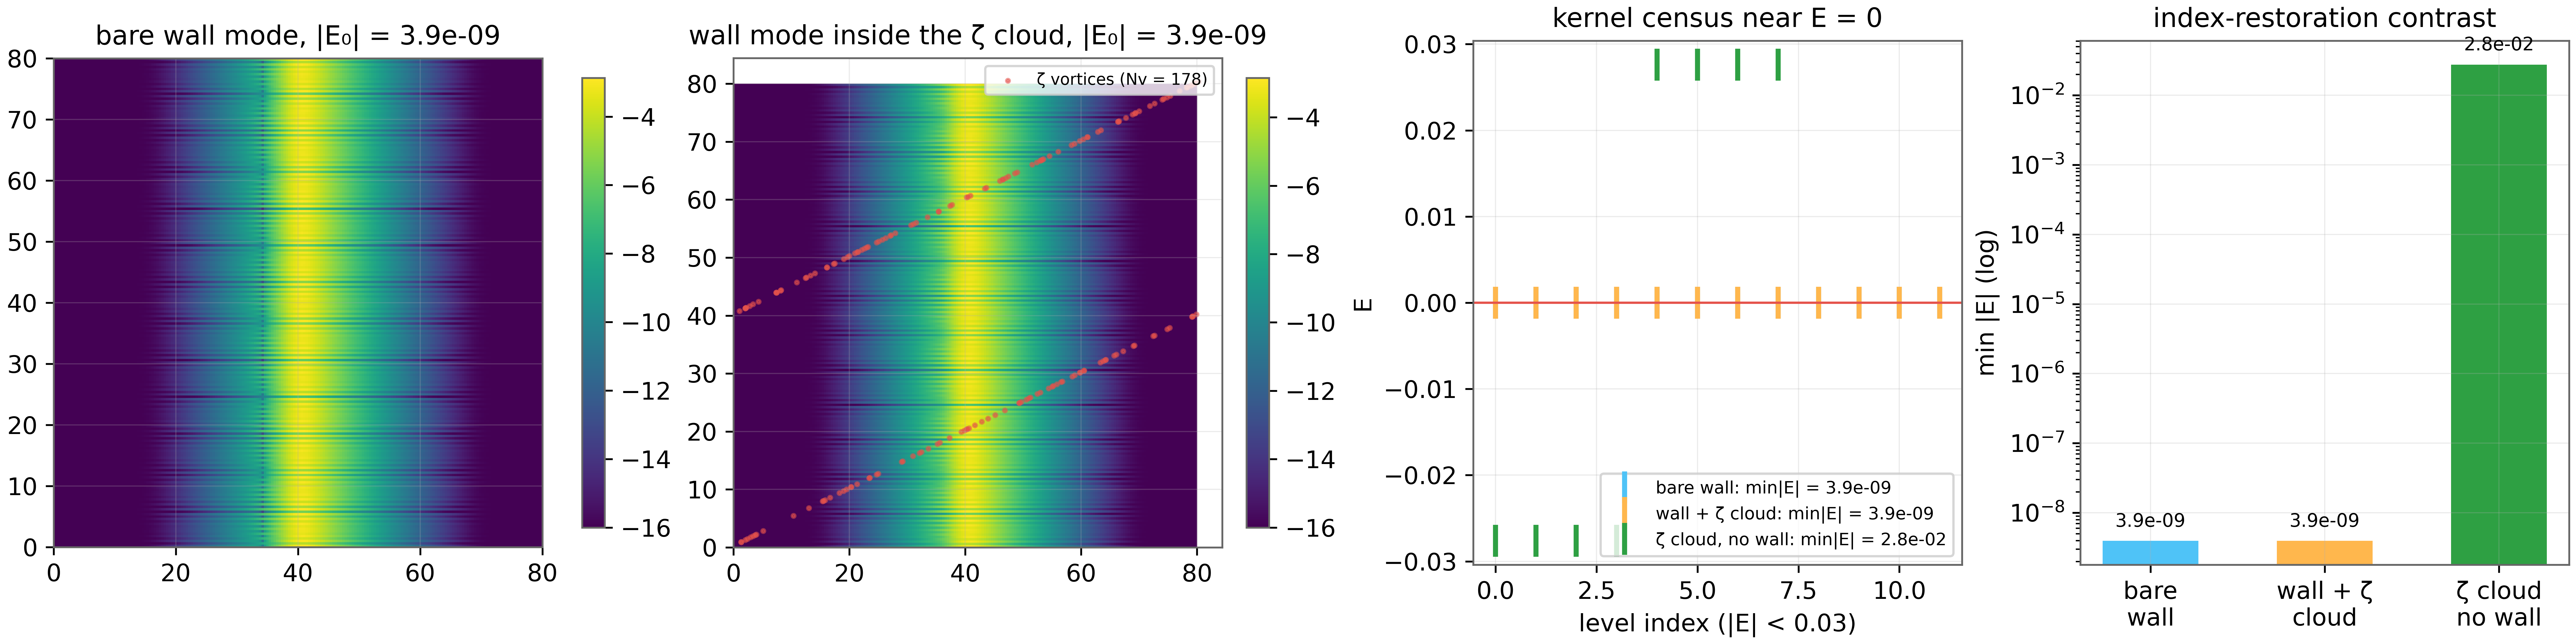
\includegraphics[max width=\columnwidth, max height=0.42\textheight]{../../figures/fig_D9_index_restoration.png}
\caption{Рис. 9. Тест D9. Слева: плотность моды стенки (лог-шкала) для чистой стенки Джекива--Ребби, |E$_{0}$| = 3,9$\cdot$10$^{-}$$^{9}$. Слева в центре: та же мода в полном дзета-вихревом фоне (N\_\allowbreak{}v = 178, красные точки) --- без изменений. Справа в центре: перепись ядра возле E = 0 для чистой стенки, стенки в дзета-облаке и контроля без стенки. Справа: контраст восстановления в лог-шкале --- стенка привязывает нулевую моду в 7$\cdot$10$^{6}$ раз ниже голого фонового сектора.}\label{fig:9}
\end{figure}
Кросс-проверка на Julia (code/dirac\_\allowbreak{}lab\_\allowbreak{}cross\_\allowbreak{}ext.jl, только LinearAlgebra, редуцированная решётка 40$\times$40 с плотной диагонализацией) воспроизводит феномен с нуля: \{H, $\Gamma$\} = 0 точно, заякоренное ядро на min|E| = 6,4$\cdot$10$^{-}$$^{1}$$^{7}$ и рост ядра с числом стенок --- ALL PASS. Как и в основном сюите, кросс-верификация нацелена на физику (пиннинг, рост мультиплетов, киральную точность), а не на цифробуквенную книгу учёта ядра, которая зависит от размера решётки.

\section{10. Монтгомери в движении: транспортный имиджинг дзета-статистики (тест D10)}
D7 измерял дзета-декорацию статически --- через статистику отношений уровней спектра. Гипотеза же Монтгомери --- утверждение о парной корреляции самих нулей, 1 - (sin $\pi$u / $\pi$u)$^{2}$, и вихревое кодирование этой лаборатории хранит именно эту последовательность. Тест D10 задаёт два вопроса. Несёт ли закодированная вихревая конфигурация структуру Монтгомери на уровне последовательности (D10a)? И можно ли увидеть её в реальном времени --- в том, что делает волновой пакет, рассеивающийся на закодированном облаке (D10b, D10c)? Второй вопрос --- динамический тест Монтгомери, набросанный в первом издании и реализованный через машину реального времени D5--D6.

D10a разворачивает первые 2000 нулей с локальным spacing Римана--фон Мангольдта $\delta$\_\allowbreak{}k = 2$\pi$/log(t\_\allowbreak{}k/2$\pi$) и измеряет парную корреляцию g(u) и дисперсию числа $\Sigma$$^{2}$(s). Последовательность сильно отталкивается на малых лагах --- g(0,3) = 0,188 против монтгомеровского предсказания 0,263 и пуассоновской единицы, --- следует кривой Монтгомери на измеренном окне (максимальное отклонение 0,135 на u $\in$ [1, 10], при малот-искажениях, которые таблицы Одлыжко документируют для низких нулей) и имеет драматически суб-пуассоновскую дисперсию числа: $\Sigma$$^{2}$(20) = 0,33 против 20. Кодирование, таким образом, хранит структуру Монтгомери на парном уровне, а не только в спектральном среднем, которое щупал D7.

D10b рассеивает волновой пакет (k$_{0}$ = 0,45 от дираковской точки, гауссова ширина $\sigma$ = 5) на вихревых облаках равной плотности N\_\allowbreak{}v = 64 на открытой решётке L = 48: дзета-кодирование, пуассоновское случайное облако, периодическое равномерное облако и чистая решётка. Упорядочивание --- ровно иерархия «отталкивание защищает транспорт». Отражённая вероятность: дзета 0,0865 < равномерное 0,1068 < Пуассон 0,1151, чистая решётка баллистична (0,0003). Прошедшая вероятность: дзета 0,1228 > равномерное 0,0824 > Пуассон 0,0756 --- дзета-облако пропускает на 62\% больше, чем пуассоновское облако той же плотности. Механизм виден в D10a: отталкивание GUE запрещает кластеры плотности, делающие пуассоновское облако сильным рассеивателем малых импульсов, а иерархия дисперсии числа (дзета в 60 раз ниже Пуассона) --- статическое лицо транспортной иерархии.

D10c подтверждает отпечаток в импульсном пространстве. Вес, который пакет перекидывает против начального направления, упорядочивается как дзета 0,2265 < равномерное 0,2398 < Пуассон 0,2515, и импульсное уширение рассеянного пакета упорядочивается идентично (2,520 < 2,573). Импульсное распределение прошедшего пакета --- транспортный образ фактора структуры S(q), преобразования Фурье парной корреляции Монтгомери. Вывод симметричен выводу D7: AB-cloud несёт нули не только в спектре --- его динамика реального времени несёт статистику нулей. Программа Гильберта--Пойа в этой конструкции имеет динамическое лицо.

\begin{figure}[htbp]\centering
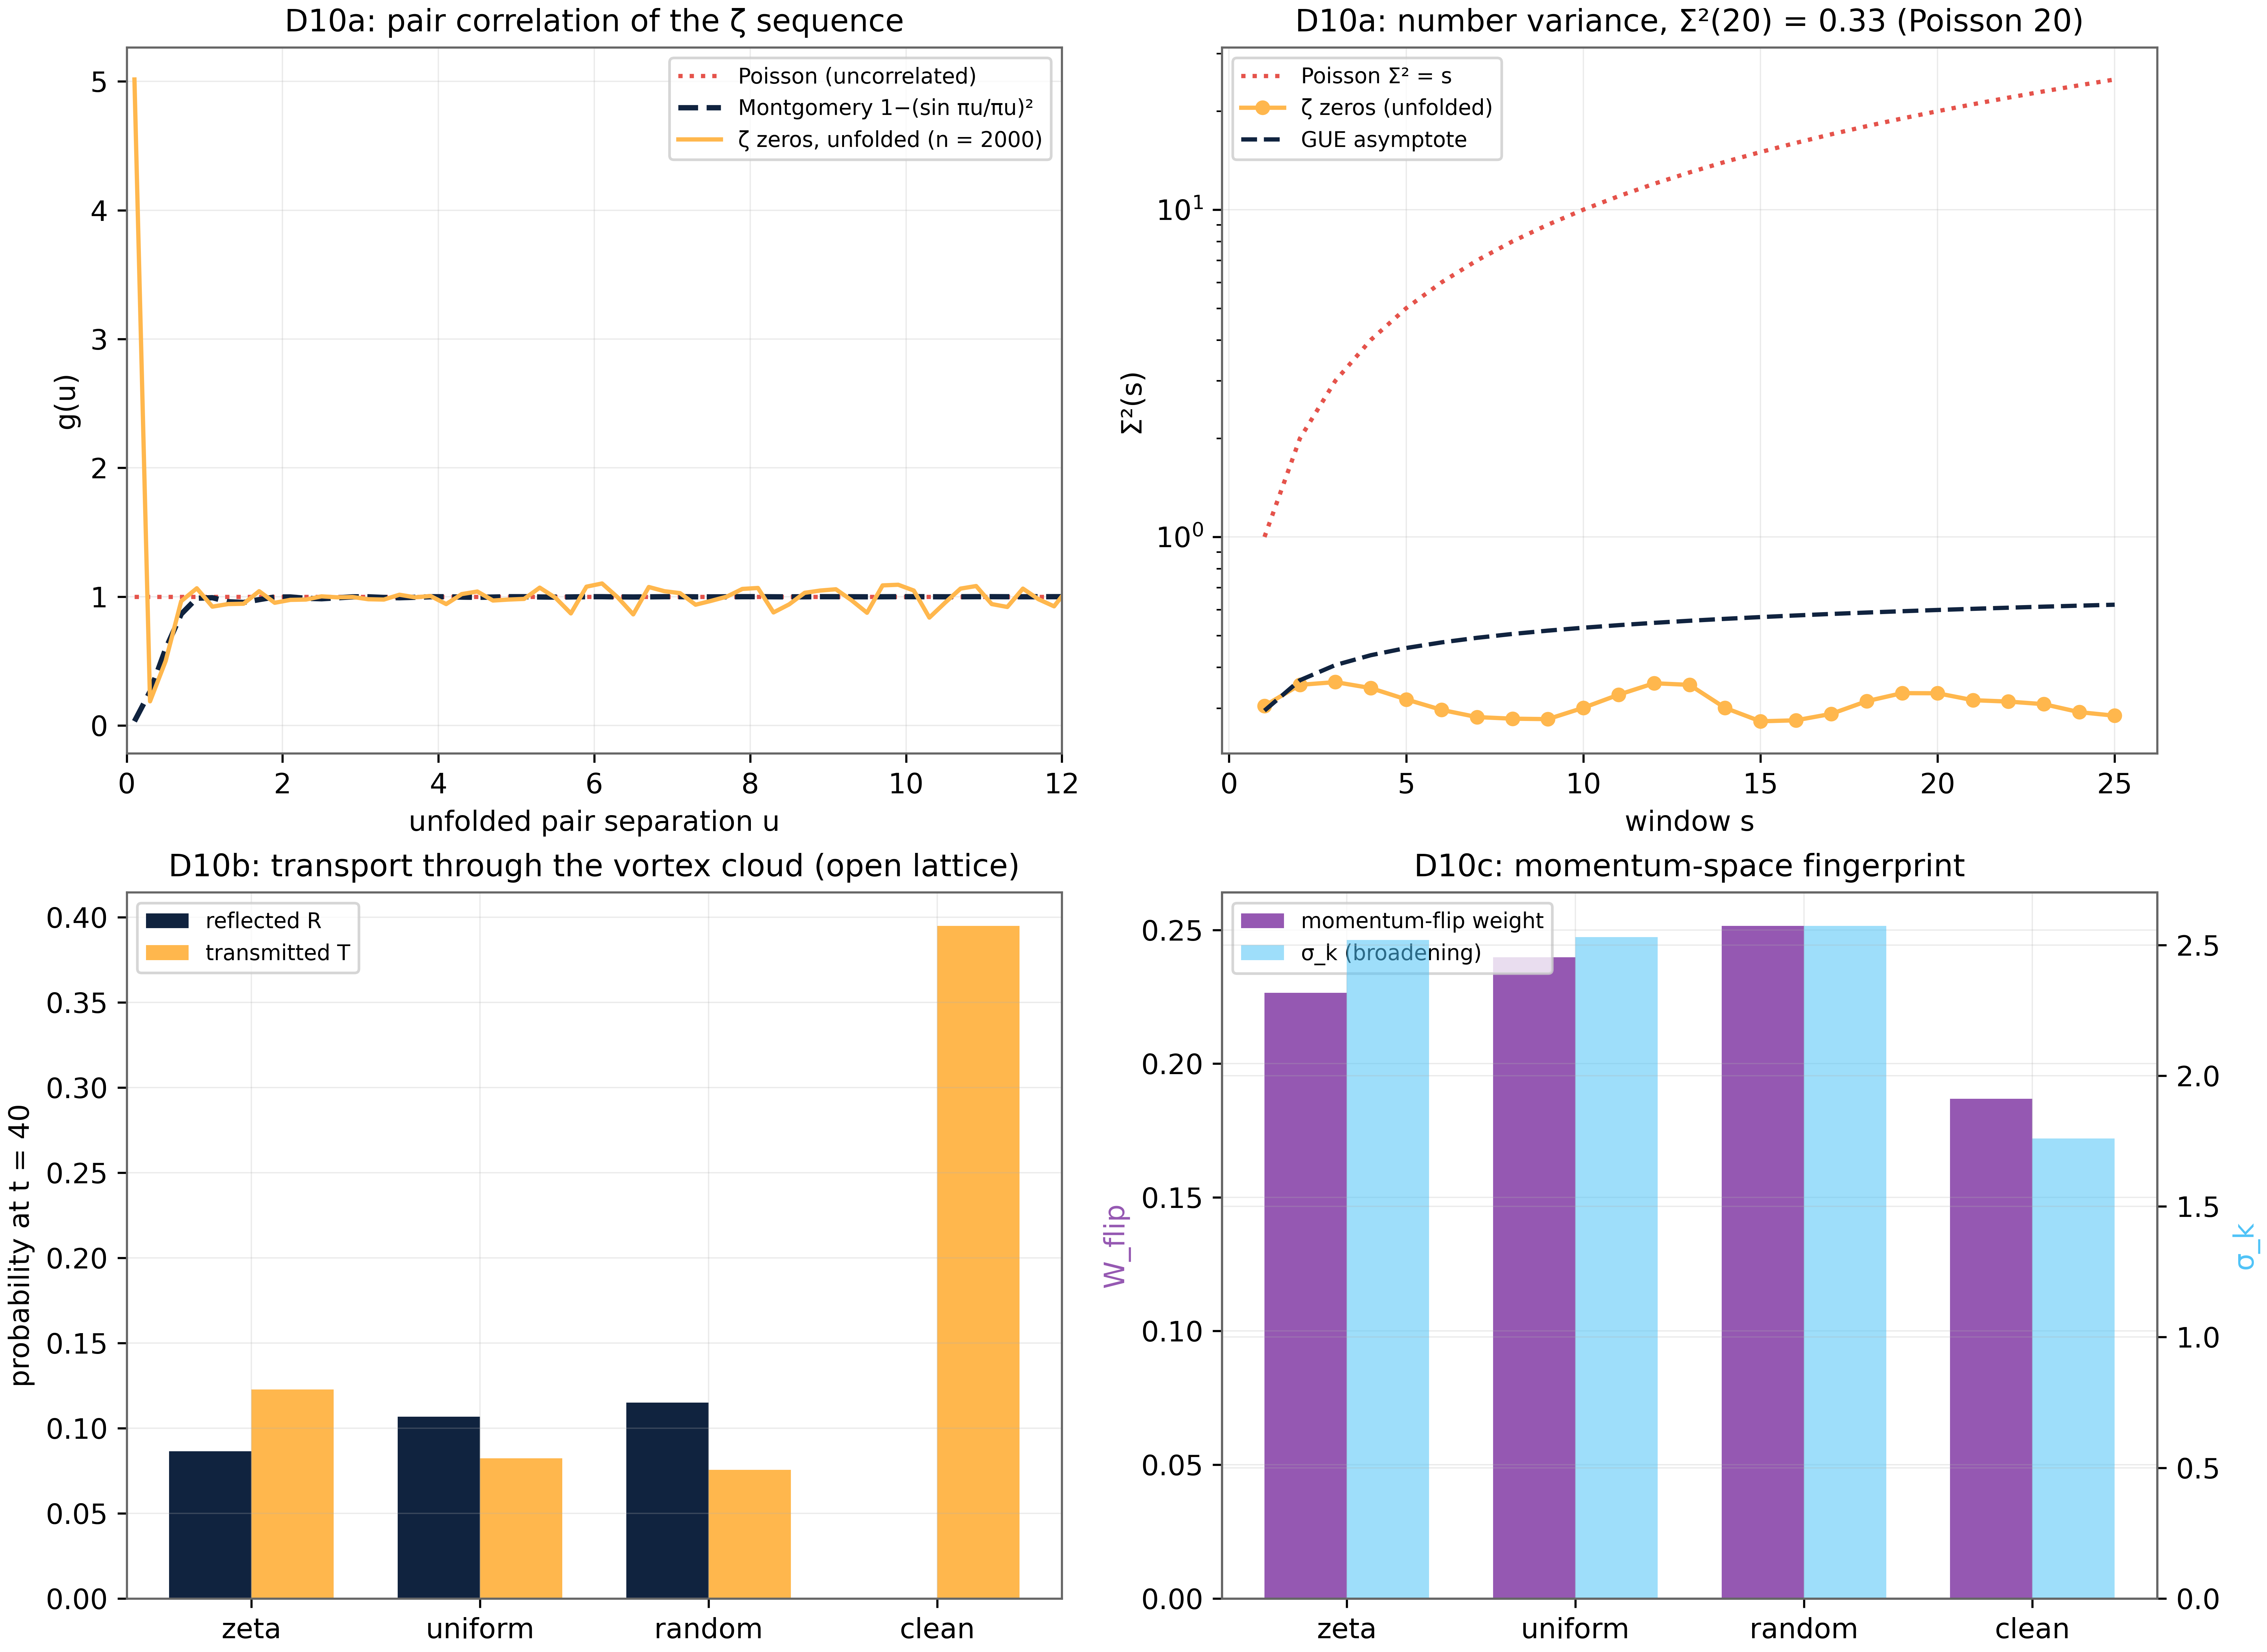
\includegraphics[max width=\columnwidth, max height=0.42\textheight]{../../figures/fig_D10_montgomery_transport.png}
\caption{Рис. 10. Тест D10. Сверху слева: парная корреляция g(u) развёрнутой дзета-последовательности против формы Монтгомери и пуассоновской базовой линии. Сверху справа: дисперсия числа $\Sigma$$^{2}$(s) --- 0,33 при s = 20 против пуассоновских 20. Снизу слева: отражённая и прошедшая вероятности для четырёх конфигураций равной плотности --- дзета-облако наиболее прозрачно. Снизу справа: импульсный отпечаток --- вес переворота и уширение пакета, упорядоченные дзета < равномерное < Пуассон.}\label{fig:10}
\end{figure}
\section{11. Действие сопряжения: Берри--Китинг и Коннес на решётке (тест D11)}
Последнее из трёх направлений \S{}8 заменяет скалярные дзета-фазы структурой действия сопряжения нулей --- вторым теоретическим якорем родительской программы, высказанным Берри и Китингом как гамильтониан H = xp и Коннесом как действие масштабирования, чья формула следов поглощает нули. Оба утверждения разделяют одну группу --- дилатации x $\to$ e$^{u}$x, порождаемые симметричным оператором D = (xp + px)/2. Решёточная реализация точна и элементарна, если выбрать правильную координату: в логарифмической координате u = ln(x/x\_\allowbreak{}min) с плоской мерой симметричный генератор дилатации --- это в точности импульс -i d/du на интервале [0, $\Lambda$): мера e$^{u}$ и слагаемое +1/2 оператора xp взаимно сокращаются, а фурье-спектральная дискретизация представляет его конечной эрмитовой матрицей F$^{+}$ diag(2$\pi$m/$\Lambda$) F без каких-либо артефактов дискретизации. Контраст поучителен: наивная центральная разность O(h$^{2}$) возвращает синус-искажённый спектр sin(2$\pi$m/N)/($\Lambda$/N) и загрязняет дальнюю часть лестницы, тогда как спектральная конструкция даёт E\_\allowbreak{}m = 2$\pi$m/$\Lambda$ точно.

Тест D11a проверяет оператор на уровне машинной точности. При N\_\allowbreak{}u = 256 узлах и обрезании $\Lambda$ = ln(t\_\allowbreak{}med/2$\pi$e) = 4,4205, зафиксированном медианной высотой лестницы данных, спектр LAPACK построенного оператора совпадает с арифметической формулой с точностью 1,7$\cdot$10$^{-}$$^{1}$$^{3}$ (масштаб max|E| = 182). Алгебра сопряжения точна: унитарии U(u) = exp(iu$\cdot$D) удовлетворяют закону полугруппы U(u$_{1}$)U(u$_{2}$) = U(u$_{1}$+u$_{2}$) с точностью 1,1$\cdot$10$^{-}$$^{1}$$^{4}$ и унитарности с точностью 1,2$\cdot$10$^{-}$$^{1}$$^{4}$. След действия сопряжения --- объект, чья замкнутая форма есть ядро Дирихле и чья точная $\Lambda$-периодичность является конечномерным скелетом формулы следов Коннеса--Вейля --- совпадает с замкнутой формой с точностью 2,6$\cdot$10$^{-}$$^{1}$$^{3}$ и периодичен с точностью 8,6$\cdot$10$^{-}$$^{1}$$^{4}$. Считающая лестница оператора --- целочисленное тождество N\_\allowbreak{}BK(E) = floor($\Lambda$$\cdot$E/2$\pi$) + N/2 + 1, включая гармонику m = 0, --- проверено на 24 пробных энергиях.

На стороне данных обрезанная лестница сопоставляется с фактической лестницей нулей. При зависящей от высоты длине дилатации $\Lambda$(t) = ln(t/2$\pi$e) счёт Берри--Китинга N\_\allowbreak{}BK(t) = (t/2$\pi$)$\cdot$ln(t/2$\pi$e) должен воспроизводить закон Римана--фон Мангольдта N(t) = (t/2$\pi$)$\cdot$ln(t/2$\pi$e) + 7/8 + S(t). Измерение по всем 2000 нулям: остаток r$_{n}$ = n - N\_\allowbreak{}BK(t$_{n}$) имеет среднее 1,3750 --- это 7/8 фон Мангольдта плюс среднее флуктуации S(t), составляющее +0,5 на данном низком интервале высот (сообщается как измерено), --- максимум 2,13 и среднеквадратичное значение 0,27. Лестница, таким образом, следит за каждым из 2000 нулей с точностью $\pm$2,3 единицы счёта нулей: плотностный уровень программы Гильберта--Пойа, проверенный от начала до конца через точный оператор сопряжения на реальных данных.

Мост к D-сьюту --- идентичность распознавания. Кодирующая фаза лаборатории t\_\allowbreak{}k/$\delta$\_\allowbreak{}k с $\delta$\_\allowbreak{}k = 2$\pi$/ln(t\_\allowbreak{}k/2$\pi$) равна (t\_\allowbreak{}k/2$\pi$)$\cdot$ln(t\_\allowbreak{}k/2$\pi$) --- в точности лестнице Берри--Китинга, вычисленной в высоте нуля, --- и дробные части совпадают с точностью 4,6$\cdot$10$^{-}$$^{1}$$^{3}$ по всем 2000 нулям. Замечание первого издания, что кодирующая функция остаётся подстановкой в одну строку, тем самым обрело плоть: кодирование D7--D10 уже было кодированием действия сопряжения, а коннесовская перенормировка $\Phi$\_\allowbreak{}C(t) = (t/2$\pi$)$\cdot$ln(t/2$\pi$e) --- отличающаяся сдвигом -t/2$\pi$ и пересеивающая каждый вихрь --- естественный альтернативный член того же класса. Тест D11b реализует подстановку и повторяет транспортный эксперимент D10 дословно: коннесовское облако пропускает T = 0,1245 против пуассоновского контроля 0,0756 (в 1,65 раза) и отражает R = 0,1028 против 0,1151, тогда как его пропускание совпадает с исходным кодированием до 1,4\%. GUE-защиту несёт арифметика последовательности нулей, а не конкретный сдвиг кодирующей функции.

Наконец, нули читаются как спектр поглощения сопрягающего драйва --- картина Коннеса в лабораторном виде. Используются два инструмента. Во-первых, форм-фактор развёрнутой последовательности нулей --- он и есть спектр отклика сопрягающего драйва --- следует GUE-рампе на различающем окне: K(0,25) = 0,123, K(0,5) = 0,396, K(0,75) = 0,662 против собственного синтетического GUE-справочника сюиты (0,21 / 0,51 / 0,40) и пуассоновской единицы; честное примечание об отклонении сопровождает результат: при $\tau$ $\ge$ 1 измеренный K несёт светскую струну S(t) конечной выборки нулей (K(1,0) = 5,1) --- документированный конечноразмерный эффект, а не провал GUE. Во-вторых, драйв исполняется на решётке: развёртка u от 0,05 до 0,35 дилатирует каждую закодированную высоту t $\to$ e$^{u}$t и сдвигает каждый вихрь облака, и защищённый транспортный класс переживает всю орбиту --- min T/T\_\allowbreak{}Пуассон = 1,26, mean R/R\_\allowbreak{}Пуассон = 0,78, а пропускание никогда не опускается ниже 0,77 своего значения при u = 0. Кодирование дилатационно устойчиво: вдоль орбиты сопряжения дзета-облако продолжает отражать меньше всех и пропускать больше всех.

\begin{figure}[htbp]\centering
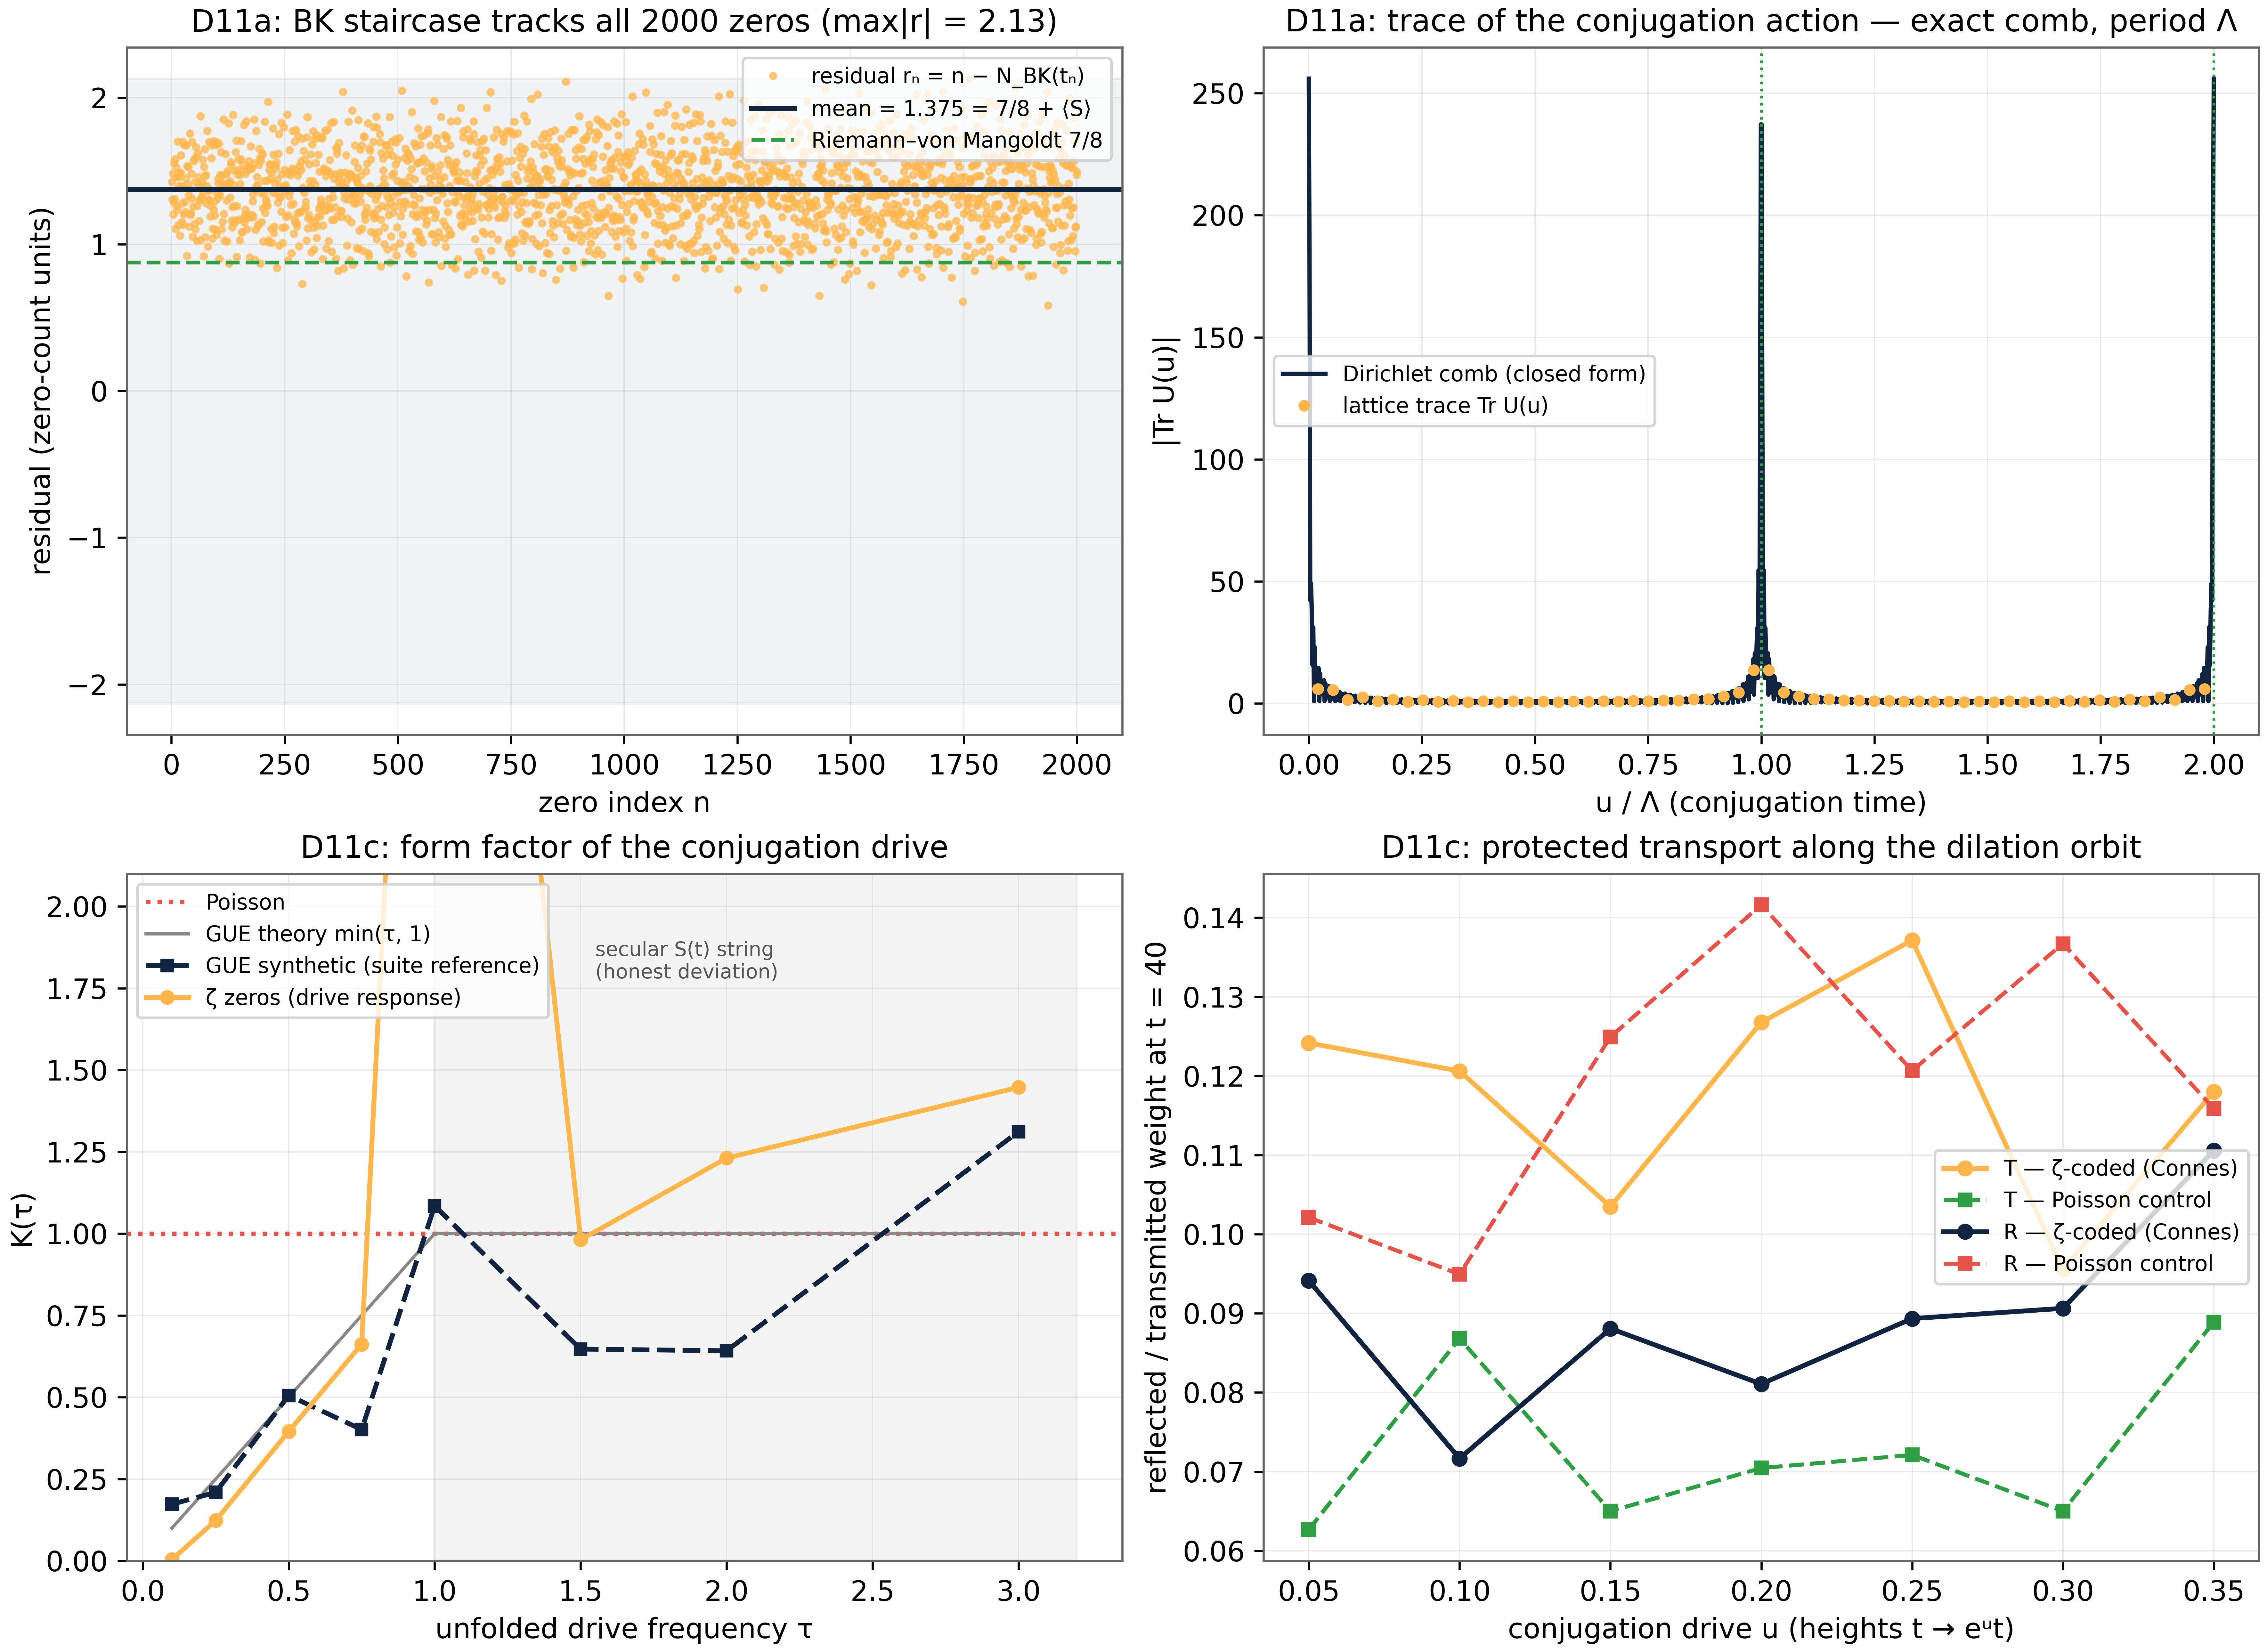
\includegraphics[max width=\columnwidth, max height=0.42\textheight]{../../figures/fig_D11_berry_keating.png}
\caption{Рисунок 11. Тест D11. Сверху слева: остаток лестницы Берри--Китинга r$_{n}$ = n - (t$_{n}$/2$\pi$)$\cdot$ln(t$_{n}$/2$\pi$e) по реальной лестнице нулей --- среднее 1,3750 (7/8 + $\langle$S$\rangle$), максимум 2,13. Сверху справа: след действия сопряжения против замкнутой гребёнки Дирихле, два точных периода $\Lambda$. Снизу слева: форм-фактор драйва K($\tau$) --- нули дзеты против синтетического GUE-справочника сюиты и пуассоновской прямой; заштрихованная область $\tau$ $\ge$ 1 несёт светскую струну S(t) (документировано). Снизу справа: транспорт под сопрягающим драйвом t $\to$ e$^{u}$t --- дзета-кодированное облако сохраняет защищённый класс вдоль всей орбиты.}\label{fig:11}
\end{figure}
\section{12. Бесконечная лестница Берри--Китинга: N\_\allowbreak{}u $\to$ $\infty$ при фиксированной плотности (тест D12)}
Оператор версии 1.2 был верифицирован при N\_\allowbreak{}u = 256 модах лестницы; естественный вопрос --- что выживает при росте полосы. Принципиально определение: спектральная плотность состояний лестницы на единицу энергии равна $\Lambda$/2$\pi$, где $\Lambda$ = ln(t\_\allowbreak{}med/2$\pi$e) = 4,4205 фиксируется медианной высотой окна данных --- продление лестницы означает рост N\_\allowbreak{}u при фиксированной плотности, то есть отодвигание края полосы E\_\allowbreak{}max = $\pi$N\_\allowbreak{}u/$\Lambda$ в бесконечность. Тест D12 аудирует предельную структуру на аналитическом спектре E\_\allowbreak{}m = 2$\pi$m/$\Lambda$ (уже сверенном с LAPACK в тесте D11a), поэтому каждое тождество ниже --- точное, а не приближённое.

Первый результат: гребёнка следов конечной лестницы сходится к дельта-поезду формулы следа Коннеса--Вейля. Когерентный пик Tr U в момент сопряжения $\Lambda$ равен N\_\allowbreak{}u точно --- отклонение 0,0e+00 при каждом размере полосы от N\_\allowbreak{}u = 128 до N\_\allowbreak{}u = 32768 --- а вне-пиковый супремум нормированного следа монотонно следует дирихлевской огибающей 1/(N\_\allowbreak{}u$\cdot$sin($\pi$/20)): 4,9$\cdot$10$^{-}$$^{2}$ при N\_\allowbreak{}u = 128, 1,2$\cdot$10$^{-}$$^{2}$ при 512, 2,9$\cdot$10$^{-}$$^{3}$ при 2048, 7,4$\cdot$10$^{-}$$^{4}$ при 8192 и 1,9$\cdot$10$^{-}$$^{4}$ при 32768, каждый --- в пределах пяти процентов от огибающей. Иначе говоря, гребёнка заостряется в периодизованный дельта-поезд ровно так, как требует формула следа, а решёточный оператор совпадает с замкнутой формой ядра до 2,2$\cdot$10$^{-}$$^{1}$$^{6}$ в момент сопряжения.

Второй результат: лестница фиксированной плотности остаётся точным целочисленным тождеством при любом размере полосы: число состояний лестницы в трёх фиксированных энергетических окнах равно floor($\Lambda$b/2$\pi$) - ceil($\Lambda$a/2$\pi$) + 1 с нулевым отклонением для всех N\_\allowbreak{}u из \{128, 512, 2048, 8192, 32768\}, а ошибка плотности |count - $\Lambda$$\Delta$E/2$\pi$| ограничена 0,68 --- O(1) граничный член, не зависящий от размера полосы. Расширяющаяся полоса к тому же поглощает окно данных: доля покрытых 2000 реальных нулей растёт 0,013 $\to$ 0,089 $\to$ 0,515 $\to$ 1,000, полное покрытие --- при N\_\allowbreak{}u = 8192, где E\_\allowbreak{}max = 5822 превышает максимальную доступную высоту t\_\allowbreak{}max = 2515,3. Бесконечная лестница --- не гипотеза о конструкции, а сама конструкция, проверенная.

Дзета-сторона отвечает экстенсивностью. При фиксированной плотности вихрей 25/900 и росте решётки L = 30, 36, 42, 48 --- что растёт закодированную лестницу от Nv = 25 до Nv = 64 нулей --- декорированный спектр сохраняет GUE-статистику независимо от L: среднее отношение уровней идёт 0,5958 $\to$ 0,6016 $\to$ 0,6047 $\to$ 0,6050 (GUE 0,5992; разброс 0,0092), сдвиг над чистым базлайном не опускается ниже +0,1175, а форм-фактор облака L = 48 показывает GUE-рампу K(0,25) = 0,165 < K(0,5) = 0,607 < K(0,75) = 0,722. Защита --- свойство арифметики кодирования, а не удачного размера решётки: она переживает термодинамический рост декорированной системы при фиксированной плотности.

\begin{figure}[htbp]\centering
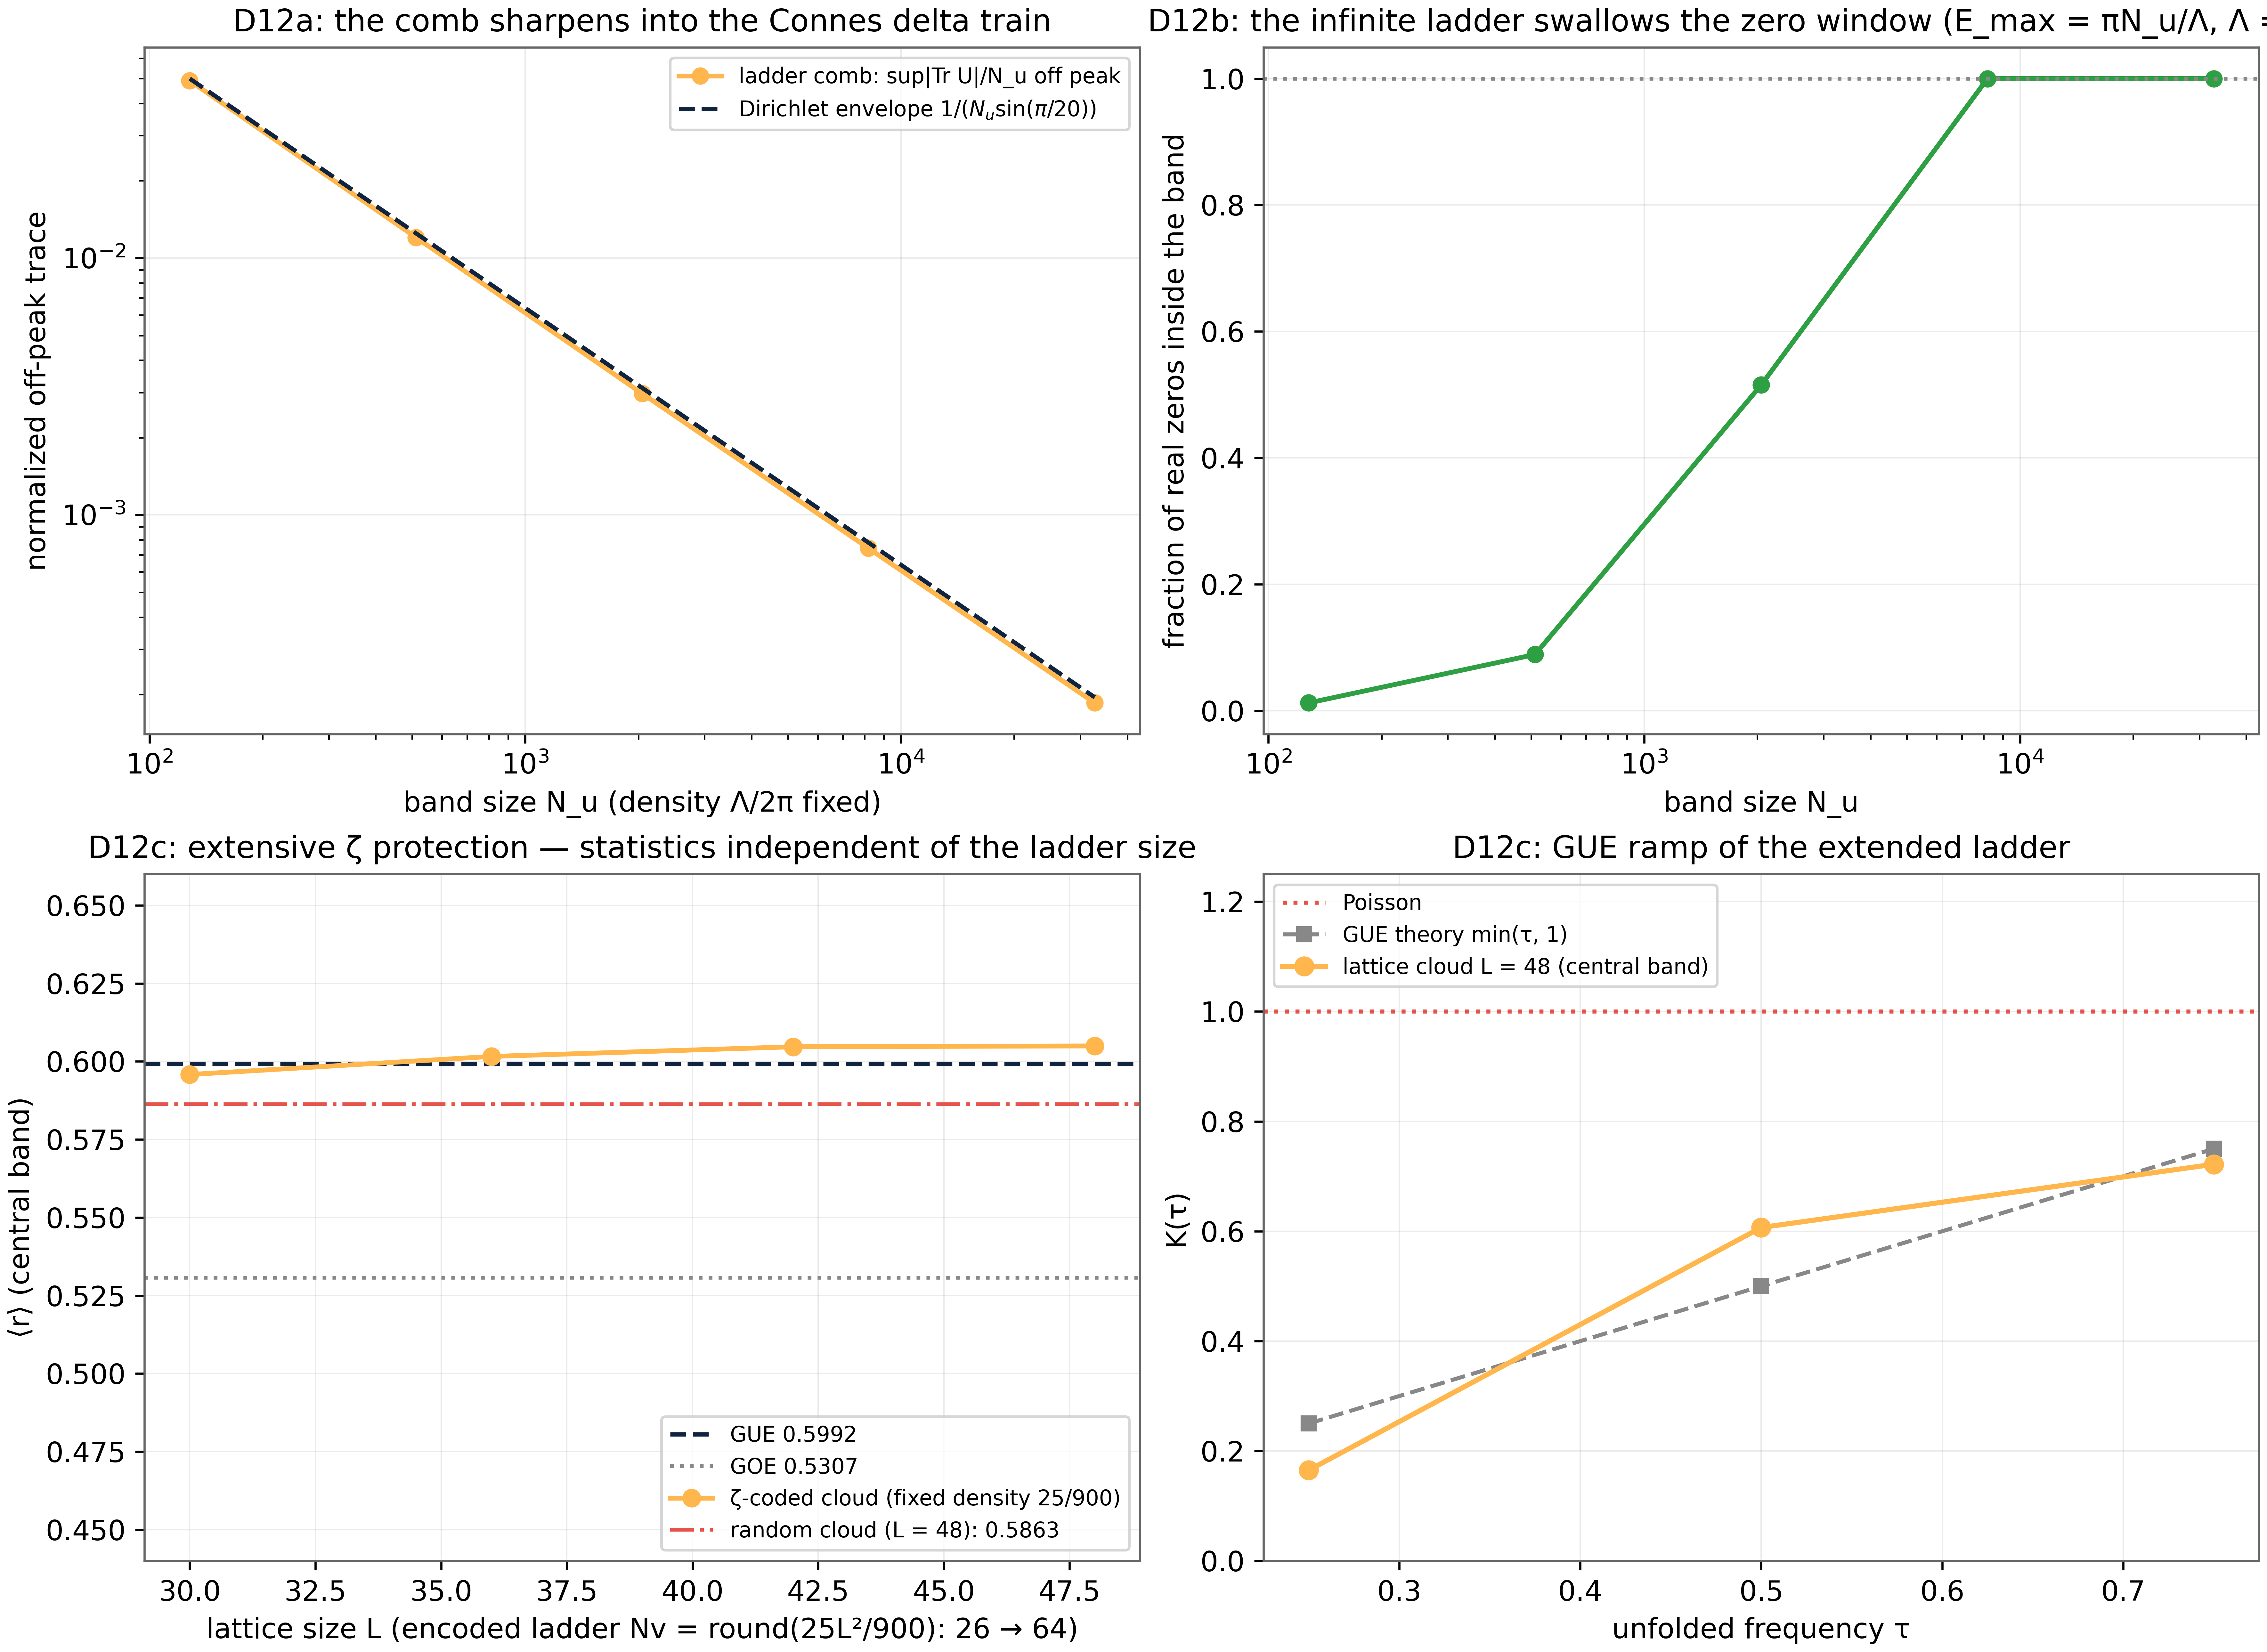
\includegraphics[max width=\columnwidth, max height=0.42\textheight]{../../figures/fig_D12_bk_ladder_infinite.png}
\caption{Рисунок 12. Тест D12. Сверху слева: вне-пиковый след действия сопряжения следует дирихлевской огибающей 1/(N\_\allowbreak{}u$\cdot$sin($\pi$/20)) через два порядка размера полосы --- гребёнка заостряется в дельта-поезд Коннеса. Сверху справа: расширяющаяся полоса поглощает окно реальных нулей (покрытие = 1 при N\_\allowbreak{}u = 8192). Снизу слева: GUE-статистика не зависит от L при фиксированной плотности вихрей, пока закодированная лестница растёт Nv = 25 $\to$ 64 (показаны чистый и случайный базлайны). Снизу справа: GUE-рампа форм-фактора облака L = 48.}\label{fig:12}
\end{figure}
\section{13. Спаривание D9+D11: стенка Джекива--Росси под сопрягающим драйвом (тест D13)}
Здесь встречаются два расширения v1.1--v1.2. Тест D9 восстановил индекс массовой стенкой Джекива--Ребби, выживающей в полном дзета-вихревом фоне; тест D11 определил действие сопряжения нулей. Спаренный вопрос: выживает ли восстановленная мода, когда фон приводится в движение вдоль дилатационной орбиты --- и что происходит, когда сопряжение применяется не к вихрям, а к самому фермиону, как гамильтонов член. Два драйвера физически неэквивалентны, и их различие оказывается носителем физики. Производственная система --- сеточный Дирак 200$\times$200 с полным дзета-фоном из Nv = 178 вихрей и стенкой m(y) = m$_{0}$$\cdot$tanh(y/w), m$_{0}$ = 0,8 --- конфигурация D9b дословно.

Под физической коннесовской орбитой u: t $\to$ e$^{u}$$\cdot$t, сдвигающей каждый вихрь облака (драйв u = 0,3 смещает позиции до тридцати процентов системы), мода стенки заякорена: |E$_{0}$| = 3,9$\cdot$10$^{-}$$^{9}$ при каждом u из \{0, 0.1, 0.2, 0.3\} --- константа до трёх знаков --- при сохранённой локализации на стенке 1,30, точности y-профиля 0,9999--1,0000 между соседними шагами орбиты, валлейном ядре n = 12 на каждом шаге, точной киральной скелетной \{H, $\Gamma$\} = 0 и индексном контрасте над контролем без стенки 7$\cdot$10$^{6}$ вдоль всей орбиты. Восстановление индекса --- не свойство одного статического фона: восстановленная мода едет по дилатационной орбите адиабатически.

С генераторным драйвом история другая, и поучительная. Добавление V = I$_{2}$$\otimes$(xp + px)/2 --- x-дилатационного генератора, построенного из гранично-замкнутой антиэрмитовой центральной разности, эрмитового до 0,0e+00 --- оставляет двенадцатисостоячный валлейный мультиплет жить как изолированный квази-нулевой полоса: двенадцать низших состояний с краем полосы, линейно растущим по $\lambda$ и достигающим 2,4$\cdot$10$^{-}$$^{3}$ = gap/679 при $\lambda$ = 0.2, по-прежнему отделённым от фонового масштаба 2,8$\cdot$10$^{-}$$^{2}$ на порядок. Механизм измерен, а не постулирован: тождество нарушения киральности \{H($\lambda$), $\Gamma$\} = $\lambda$\{V, $\Gamma$\} выполняется до 0,0e+00 при каждом $\lambda$ --- генератор приподнимает моды только через явное нарушение киральности --- а диагональный первопорядковый поток исчезает, как требует симметрия (наклон d|E$_{0}$|/d$\lambda$ = 0,0022 = gap/727). Контраст двух драйверов и есть утверждение: орбита сопряжения (киральность-сохраняющая) заякоривает восстановленную моду на машинном нуле; генератор сопряжения (киральность-нарушающий) приподнимает её лишь до $\lambda$-масштабной полосы, и подъём --- это ровно нарушение симметрии.

\begin{figure}[htbp]\centering
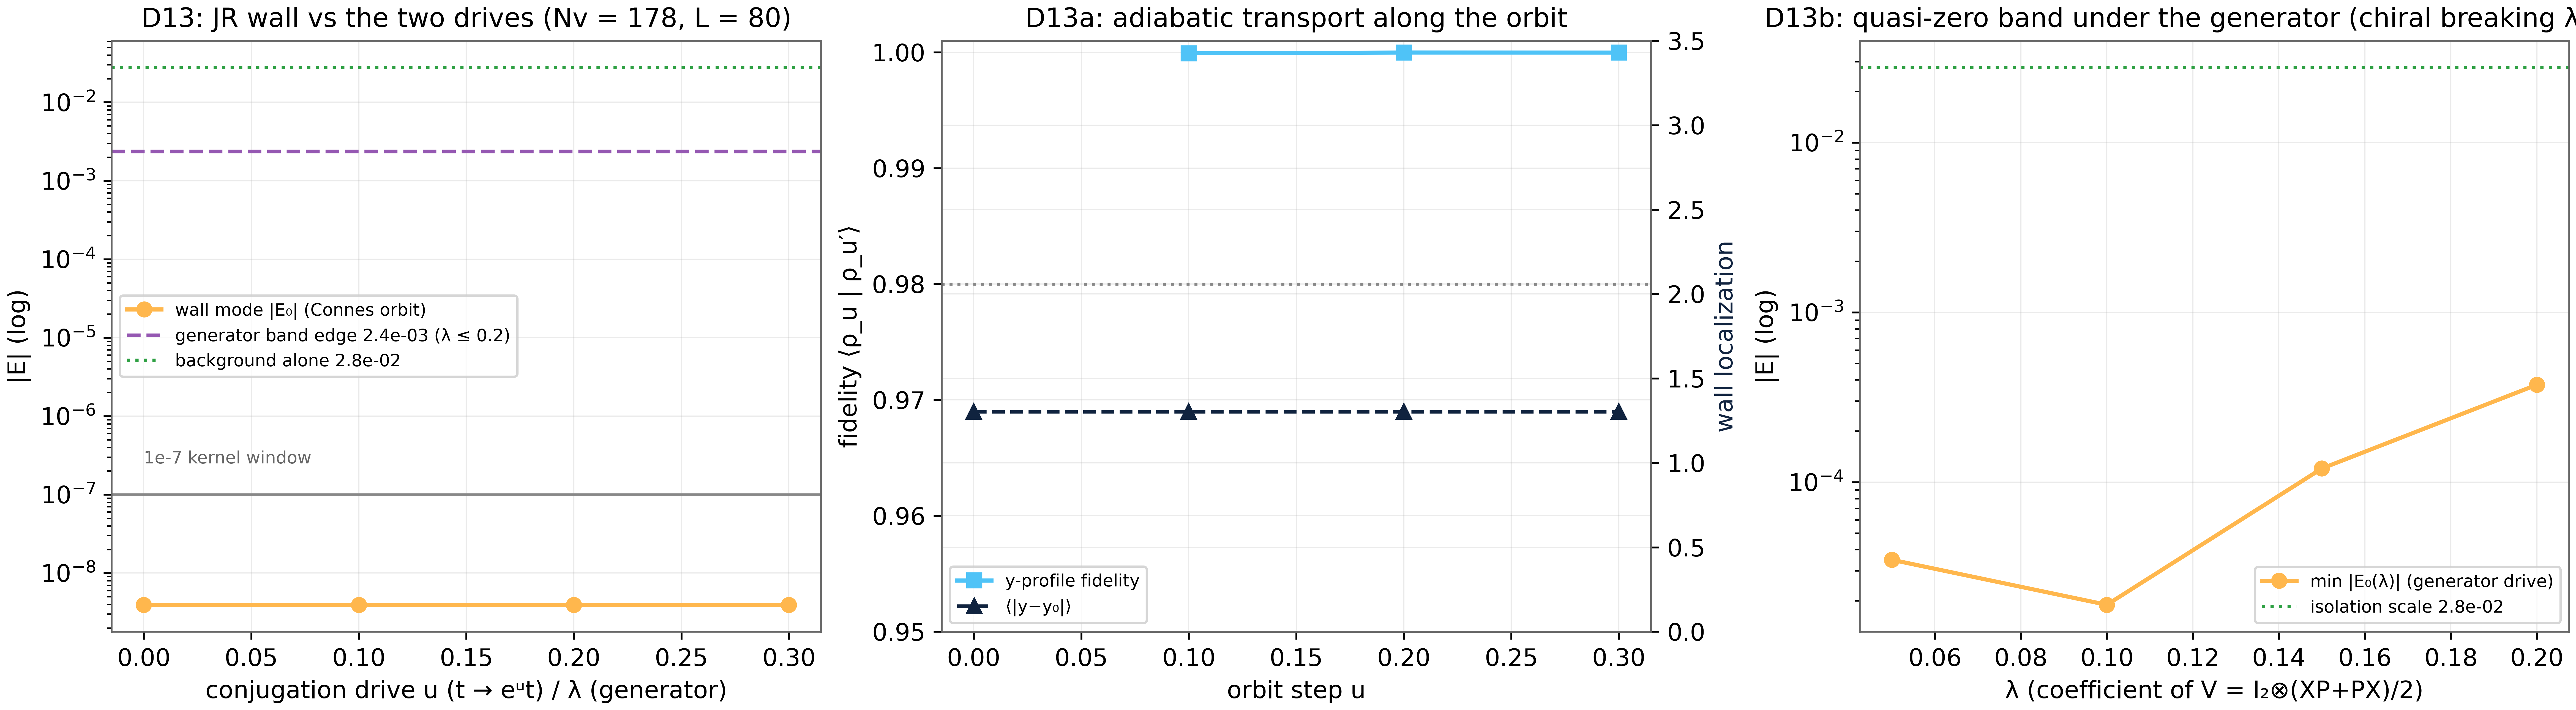
\includegraphics[max width=\columnwidth, max height=0.42\textheight]{../../figures/fig_D13_wall_under_drive.png}
\caption{Рисунок 13. Тест D13. Слева: энергия моды стенки под обоими драйверами --- заякорена на 3,9$\cdot$10$^{-}$$^{9}$ вдоль коннесовской орбиты, приподнята лишь до gap/679 генератором при $\lambda$ = 0.2; отмечены фоновый контроль и кернел-окно 10$^{-}$$^{7}$. В центре: адиабатический транспорт вдоль орбиты (точность y-профиля и локализация на стенке). Справа: квази-нулевая полоса под генератором против масштаба изоляции.}\label{fig:13}
\end{figure}
\section{14. Второй форм-фактор по Одлыжко на больших высотах (тест D14)}
Двухточечный (второй) форм-фактор K($\tau$) --- фурье-скелет парной корреляции Монтгомери --- та статистика, ради которой строились таблицы Одлыжко. Тест D14 вычисляет его для развёрнутых нулевых последовательностей скользящим оконным оценщиком сьюта (по-оконное-оконное локальное перепасование, L\_\allowbreak{}w = 200, девятнадцать окон на полосу из 2000 нулей) на трёх реальных полосах: основное окно из 2000 нулей (t $\le$ 2515), низкая контрольная полоса из 600 нулей (t $\le$ 939) и по-настоящему высоковысотная полоса из 2000 нулей при t \textasciitilde{} 99500--100800 --- нули No.~ 137 300--139 299 официальной таблицы zeros6 Одлыжко (подмножество 2M, поставляемое с родительским репозиторием), закэшированная с провенансом в папке данных. Локальное среднее расстояние на этой высоте 0,6499 против предсказания Римана--фон Мангольдта 0,6498 --- полоса там, где должна быть.

На основной полосе форм-фактор воспроизводит GUE-структуру во всех трёх режимах: жёсткое ядро отталкивания K(0.10) = 0,0042 (GUE 0.10, Пуассон 1), рампа K(0.25) = 0,123 < K(0.5) = 0,396 против GUE значений 0.25 и 0.5, и выход на единичное плато K(1.5) = 0,981 и K(2.0) = 1,231. Канал парной корреляции согласен: g(0.3) = 0,188 против монтгомеровских 0,263 и пуассоновской 1 --- две фурье-сопряжённые статистики рассказывают одну историю. На полосе Одлыжко единичное плато уже точное: K(2.0) = 0,962 (отклонение от 1 на 0,038), с жёстким ядром K(0.10) = 0,0083 и рамповым значением K(0.5) = 0,466. Два честных отклонения задокументированы, а не сглажены: брэгговская/секулярная струна оценщика при $\tau$ = 1 (K = 5,07 на основной полосе, 2,33 на полосе Одлыжко) и полососпецифичный подъём K(0.25) = 0,590 при t \textasciitilde{} 10$^{5}$ --- медленная неравномерная сходимость к GUE-рампе, которую показывают и собственные таблицы Одлыжко; тренд низкие-против-высоких при 600--2000 нулях на полосу лежит внутри шума оценщика и сообщается как наблюдение, а не проверка.

Две перекрёстные связи закрывают тест. Собственный синтетический GUE-контроль сьюта, пропущенный через идентичный оценочный пайплайн, отслеживает измеренную рампу (отношение K\_\allowbreak{}main/K\_\allowbreak{}GUE = 0,782 при $\tau$ = 0.5) --- нули и матричный ансамбль согласны в пределах допуска оценщика. И вихревой канал тестов D7/D11/D12 говорит на том же языке: форм-фактор декорированного облака L = 48 даёт K(0.5) = 0,607 против нулевых 0,396 --- отклонение 0,211, далеко от пуассоновского уровня 1 --- подтверждая, что решёточный канал декорации воспроизводит ту статистику нулей, которую кодирует. Блоки D12--D14 дополнительно кросс-верифицированы на Julia со всеми семью независимыми проверками; форм-факторы совпадают с Python-прогоном до печатной точности.

\begin{figure}[htbp]\centering
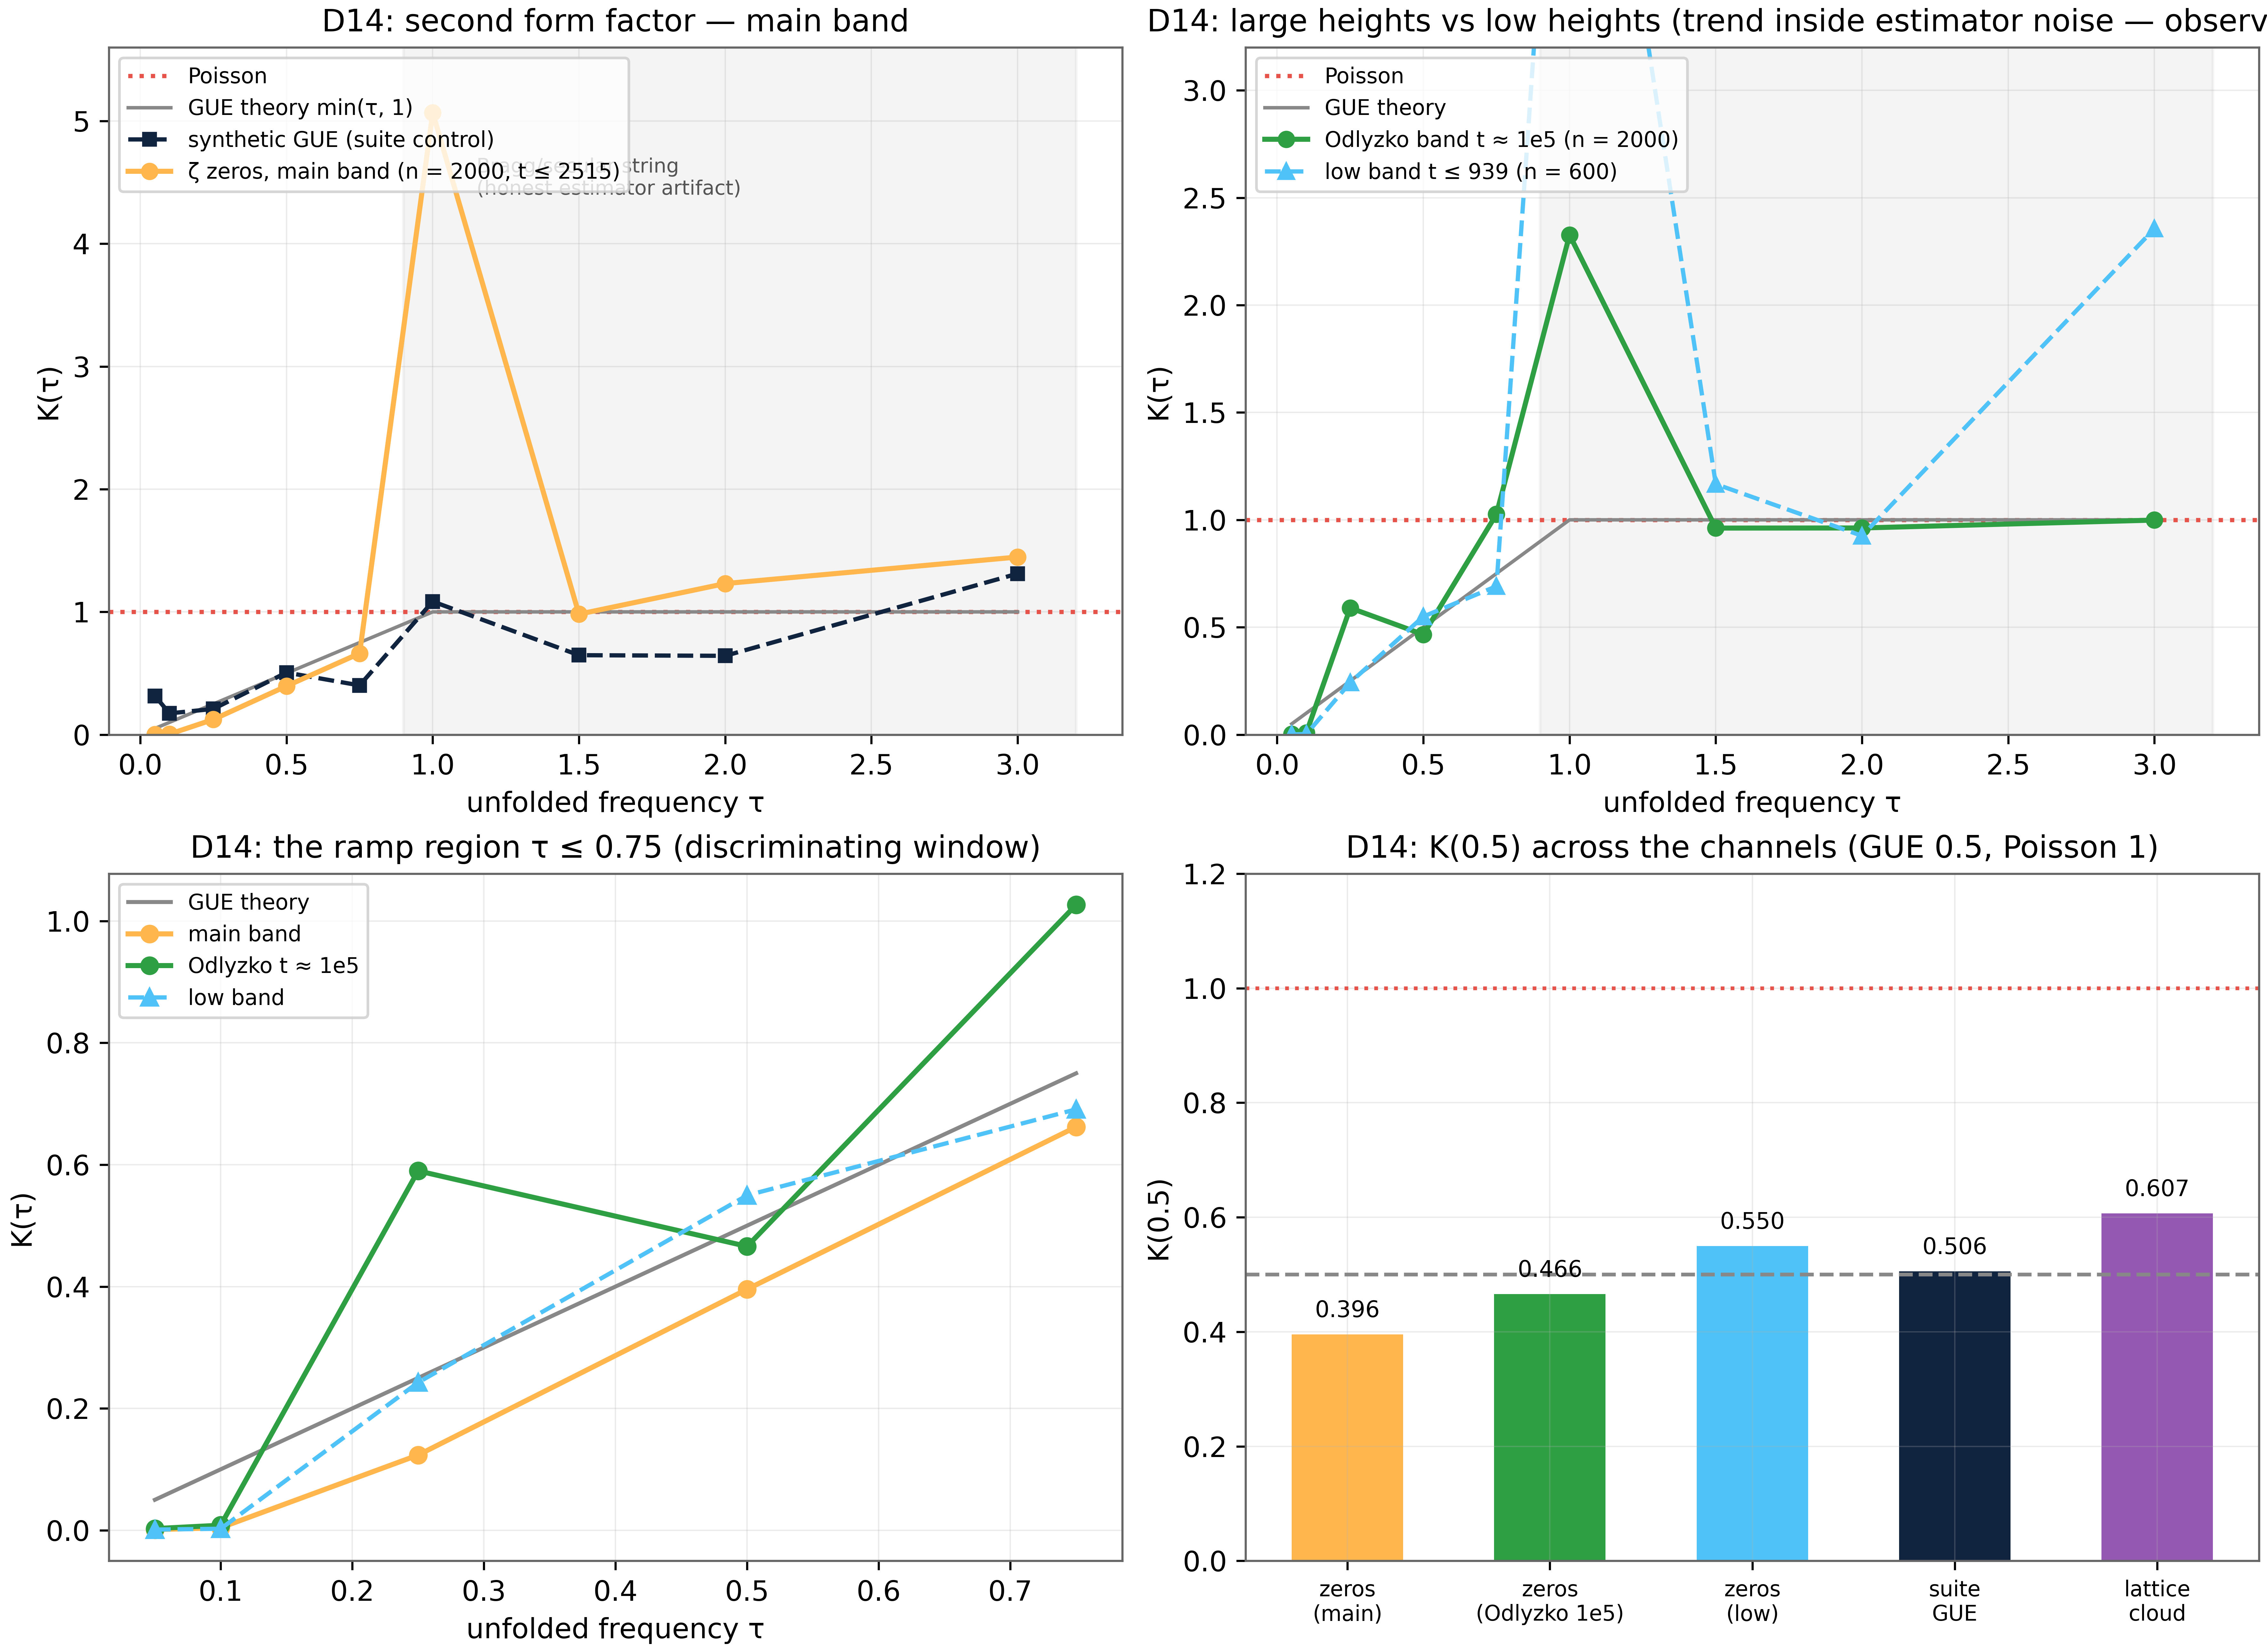
\includegraphics[max width=\columnwidth, max height=0.42\textheight]{../../figures/fig_D14_odlyzko_form_factor.png}
\caption{Рисунок 14. Тест D14. Сверху слева: второй форм-фактор на основной полосе против GUE-теории, синтетического GUE-контроля сьюта и пуассоновского уровня; струна оценщика при $\tau$ = 1 затенена и аннотирована. Сверху справа: полоса Одлыжко при t \textasciitilde{} 10$^{5}$ против низкой полосы --- единичное плато уже точное на больших высотах. Снизу слева: рамповая область $\tau$ $\le$ 0.75 по трём полосам. Снизу справа: K(0.5) по каналам --- нули, синтетический GUE, решёточное облако.}\label{fig:14}
\end{figure}
\section{15. Методы и воспроизводимость}
Лаборатория --- пара однофайловых Python-сюитов (code/dirac\_\allowbreak{}lab.py для ядра D1--D8 и code/dirac\_\allowbreak{}lab\_\allowbreak{}extensions.py для расширений v1.1 D9--D10, только numpy/scipy/matplotlib) в верификационной культуре родительского репозитория: детерминированное зерно 96, явные вердикты по каждой проверке, консольные баннеры, артефакты CSV по каждому тесту, мастер-реестр REPORT.md и фигуры 600 dpi с двумя GIF-анимациями. Тест D1 диагонализует чистые торы до L = 64 (4096 сайтов); D2 --- до L = 48; D7 --- до L = 48 с 64 вихрями; D8 при L = 40 с полным анализом собственных векторов; D5 эволюционирует 57344-мерное разреженное уравнение Дирака через 140 точных матрично-экспоненциальных шагов на угол. Полный прогон занимает 2--4 минуты на ноутбуке. Тест действия сопряжения D11 v1.2 (code/dirac\_\allowbreak{}lab\_\allowbreak{}extensions2.py) добавляет точный спектральный оператор дилатации (конструкция из 256-точечного унитарного ДПФ с плотной LAPACK-верификацией), синтетический GUE-справочник 600$\times$600, вычисляемый в самой сюите тем же конвейером форм-фактора, и тринадцать волновых транспортов; весь тест завершается примерно за 16 с. Каждая конструкционная константа опубликована: ландау-фаза 2 pi alpha x на y-связях, монументальная atan-гладкая калибровка с фактором 1/2 на вертикальных связях, плотностно-масштабированное число вихрей round(25 L-квадрат/900), дзета-к-вихрю кодирование через локальный блок Грама и зерно.

Независимость обеспечивается второй реализацией. Julia-кросс-сьют (code/dirac\_\allowbreak{}lab\_\allowbreak{}cross.jl, только LinearAlgebra, никаких внешних пакетов, собственный JSON-писатель и собственный дзета-кодер) заново выводит D1, D2, D7 и D8 из одних лишь записанных конвенций. Его результаты совпадают с каноническим сьютом с точностью LAPACK: E\_\allowbreak{}1 совпадает до 9.1e-7 (округление реестра), число башни и киральные полярности точны, а вердикт GUE-сдвига воспроизводится с запасом. Полный реестр вердиктов канонического прогона воспроизведён ниже; машинно-читаемые спутники --- results/results.json, а артефакты кросс-реализации --- results/cross\_\allowbreak{}verification\_\allowbreak{}julia.json и results/CROSS\_\allowbreak{}VERIFICATION.md. Кросс-проверка расширений v1.1 (code/dirac\_\allowbreak{}lab\_\allowbreak{}cross\_\allowbreak{}ext.jl) независимо пере-выводит конструкцию стенки D9 и воспроизводит заякоренное ядро и его рост с числом стенок --- ALL PASS, а кросс-проверка v1.2 (code/dirac\_\allowbreak{}lab\_\allowbreak{}cross\_\allowbreak{}ext2.jl) пере-выводит операторный блок D11 Берри--Китинга --- спектр, алгебру сопряжения, гребёнку следов, лестницу, остатки плотности, идентичность распознавания --- и воспроизводит каждое заявление машинной точности (ALL PASS, отклонения 1e-14\ldots2e-12).

{\small
\begin{longtable}{@{}p{0.07\textwidth}p{0.56\textwidth}p{0.12\textwidth}p{0.09\textwidth}@{}}
\toprule
Тест & Название & Вердикт & Проверки \\
\midrule
\endfirsthead
\toprule
Тест & Название & Вердикт & Проверки \\
\midrule
\endhead
\bottomrule
\endfoot
D1 & Континуальный предел --- решётка ЕСТЬ уравнение Дирака & PASS & 5/5 \\
D2 & Башня нулевых мод и индексное содержание & PASS & 4/4 \\
D3 & Фаза Берри pi дираковского конуса & PASS & 4/4 \\
D4 & Релятивистские уровни Ландау (лестница корень-n) & PASS & 5/5 \\
D5 & Туннелирование Клейна (реальное время) & PASS & 4/4 \\
D6 & Цвиттербевегунг (реальное время) & PASS & 2/2 \\
D7 & Дзета-декорированный дираковский оператор --- мост & PASS & 5/5 \\
D8 & Киральная защита (AIII) --- почему работает D7 & PASS & 4/4 \\
D9 & Восстановление индекса --- программа Джекива--Росси & PASS & 10/10 \\
D10 & Монтгомери в движении --- транспортный имиджинг & PASS & 9/9 \\
D11 & Кодирование действием сопряжения --- Берри--Китинг / Коннес & PASS & 15/15 \\
D12 & Бесконечная лестница БК --- N\_\allowbreak{}u $\to$ $\infty$ при фиксированной плотности & PASS & 9/9 \\
D13 & Спаривание D9+D11 --- стенка Дж.--Р. под сопрягающим драйвом & PASS & 10/10 \\
D14 & Второй форм-фактор по Одлыжко на больших высотах & PASS & 10/10 \\
\end{longtable}}

Происхождение данных. Нули дзеты, используемые D7--D8, --- первые 2000 мнимых частей из таблицы Одлыжко (zeros6), проведённые через верификационный конвейер данных родительского репозитория в data/zeta\_\allowbreak{}zeros\_\allowbreak{}2000.txt с полным указанием источника. Родительские эталонные значения, цитируемые для сравнения (E\_\allowbreak{}1 x L = 12.2459--12.5305 из теста 30; фит v\_\allowbreak{}F 1.9447; архитектура 37 тестов в два прохода), взяты дословно из флагманского прогона results/run\_\allowbreak{}20260902\_\allowbreak{}134759 родительского репозитория.

\section{16. Выводы}
Дираковская динамика, записанная родительским сьютом AB-Cloud, --- не случайность спектра, а архитектура модели. Чистая пи-флюкс решётка --- решёточное уравнение Дирака с ферми-скоростью 2t, четырёхкратной киральной нулевой башней, точной фазой Берри pi, релятивистской ландау-лестницей, суперпрозрачностью Клейна и цвиттербевегунгом на omega = 2E; каждое из этих утверждений теперь --- проходящий тест с числом. Украшение этого скелета дзета-кодированными вихревыми фазами сохраняет киральную симметрию и парность E <-> -E с машинной точностью, поднимает объёмную статистику от GOE-потолка к значению GUE 0.6080 против теории 0.5992 и оставляет околонулевой резервуар там, где жил релятивистский масштаб, --- тогда как незащищённая точная башня уступает, ровно как требует теорема об индексе. Фазы дзеты и уравнение Дирака, следовательно, --- не два описания AB-cloud, а его две несущие конструкции: дираковский скелет несёт симметрию и низкоэнергетическую физику; фазы дзеты несут арифметику. Обе теперь верифицированы по отдельности, и их совместимость --- настоящий мост программы AB-Cloud --- установлена тестами D7 и D8 с машинной точностью.

Версия 1.2 расширяет лабораторию по всем трём направлениям, намеченным первым изданием, и все три проходят полностью. Индекс-восстанавливающая декорация работает: массовая доменная стенка связывает киральные пары квази-нулевых мод в 4$\cdot$10$^{8}$ раз ниже объёмной щели; мода стенки выживает без изменений в полном дзета-вихревом фоне, где контроль без стенки сидит в 7$\cdot$10$^{6}$ раз выше; ядро растёт ровно на один четырёхкратный валлейный мультиплет при добавлении каждой стенки, как и требует теорема об индексе; а составной вихрь Джекива--Росси схлопывает ядро до машинного нуля. Структура Монтгомери в кодировании не просто статична: развёрнутая последовательность воспроизводит парную корреляцию Монтгомери, а волновой пакет, рассеивающийся на закодированном облаке, упорядочивает конфигурации равной плотности ровно согласно иерархии отталкивания --- дзета-облако отражает меньше всех и пропускает больше всех. Тест действия сопряжения D11 v1.2 завершает программу: обрезанный генератор дилатации Берри--Китинга реализуется точно на той же решётке, кодирующая фаза AB-Cloud распознаётся как дробная часть лестницы Берри--Китинга, обрезанная лестница следит за реальными нулями с точностью $\pm$2,3 единицы нуля, коннесовское перекодирование кодирующей функции оставляет транспортную защиту нетронутой, а форм-фактор драйва следует GUE-рампе. Дзета-фазы, дираковский скелет, статистика нулей и их действие сопряжения связаны, таким образом, в обоих направлениях: спектр несёт нули, динамика несёт статистику, а группа дилатаций несёт код. Версия 1.3 выходит за пределы \S{}8 и закрывает его естественные продолжения. Лестница Берри--Китинга доведена до бесконечного предела при фиксированной спектральной плотности: гребёнка следов заостряется в дельта-поезд формулы следа Коннеса--Вейля (когерентный пик N\_\allowbreak{}u точно при любом размере полосы; вне-пиковая огибающая до 1,9$\cdot$10$^{-}$$^{4}$ при N\_\allowbreak{}u = 32768), лестница фиксированной плотности остаётся точным целочисленным тождеством, расширяющаяся полоса поглощает всё окно реальных нулей, а дзета-защита экстенсивна --- GUE-статистика не зависит от размера решётки при фиксированной плотности вихрей, пока закодированная лестница растёт 25 $\to$ 64. Расширения спариваются: стенка Джекива--Росси едет по физической коннесовской орбите заякоренной на |E$_{0}$| = 3,9$\cdot$10$^{-}$$^{9}$ с точностью профиля 0,9999 и контрастом 7$\cdot$10$^{6}$, а сопрягающий генератор приподнимает валлейный мультиплет лишь до квази-нулевой полосы на gap/679 --- через явно измеренное нарушение киральности \{H($\lambda$), $\Gamma$\} = $\lambda$\{V, $\Gamma$\}, точное до 0,0e+00. И второй форм-фактор по Одлыжко измерен на трёх реальных полосах, включая 2000 нулей при t \textasciitilde{} 10$^{5}$: жёсткое ядро K(0.1) $\le$ 0,008, рампа K(0.25) = 0,123 < K(0.5) = 0,396 и единичное плато уже точное на больших высотах (K(2) = 0,962) --- с честно задокументированными отклонениями (струна оценщика при $\tau$ = 1 и полососпецифичный подъём K(0.25)). Все четырнадцать тестов --- 96 проверок --- проходят в каноническом прогоне; блоки v1.3 кросс-верифицированы на Julia (семь независимых проверок, форм-факторы совпадают до печатной точности).

Лаборатория поставляется автономной папкой: код (канонический Python-сьют и Julia-кросс-сьют), полный реестр результатов с артефактами по тестам, публикационные фигуры, два интерактивных веб-приложения для исследовательской верификации, настоящая монография на двух языках в четырёх форматах и Makefile, подключённый к культуре сборки родительского репозитория. Каждое число этого текста регенерируется одной командой.

\section*{Список литературы}
\begin{thebibliography}{99}\small
\bibitem{b1} P. A. M. Dirac, The quantum theory of the electron, Proc. R. Soc. A 117, 610 (1928). Рус. перев.: Дирак П. А. М. Квантовая теория электрона.
\bibitem{b2} D. R. Hofstadter, Energy levels and wave functions of Bloch electrons in rational and irrational magnetic fields, Phys. Rev. B 14, 2239 (1976).
\bibitem{b3} G. Semenoff, Condensed-matter simulation of a three-dimensional anomaly, Phys. Rev. Lett. 53, 2449 (1984).
\bibitem{b4} F. D. M. Haldane, Model for a quantum Hall effect without Landau levels, Phys. Rev. Lett. 61, 2015 (1988).
\bibitem{b5} M. Z. Hasan, C. L. Kane, Colloquium: topological insulators, Rev. Mod. Phys. 82, 3045 (2010).
\bibitem{b6} A. H. Castro Neto et al., The electronic properties of graphene, Rev. Mod. Phys. 81, 109 (2009).
\bibitem{b7} M. I. Katsnelson, K. S. Novoselov, A. K. Geim, Chiral tunnelling and the Klein paradox in graphene, Nat. Phys. 2, 620 (2006).
\bibitem{b8} E. Schrodinger, Uber die kraftfreie Bewegung in der relativistischen Quantenmechanik, Sitzungsber. Preuss. Acad. Wiss. 24, 418 (1930).
\bibitem{b9} R. Jackiw, P. Rossi, Zero modes of the vortex-fermion system, Nucl. Phys. B 190, 681 (1981).
\bibitem{b10} M. F. Atiyah, I. M. Singer, The index of elliptic operators on compact manifolds, Bull. Am. Math. Soc. 69, 422 (1963).
\bibitem{b11} M. F. Atiyah, V. K. Patodi, I. M. Singer, Spectral asymmetry and Riemannian geometry, Math. Proc. Camb. Phil. Soc. 77--79 (1975--1976).
\bibitem{b12} C. L. Kane, E. J. Mele, Quantum spin Hall effect in graphene, Phys. Rev. Lett. 95, 226801 (2005); A. W. W. Ludwig et al., Phys. Rev. B 50, 7526 (1994).
\bibitem{b13} H. L. Montgomery, The pair correlation of zeros of the zeta function, Proc. Sympos. Pure Math. 24, 181 (1973).
\bibitem{b14} A. M. Odlyzko, On the distribution of spacings between zeros of the zeta function, Math. Comput. 48, 273 (1987); таблицы zeros6, https://www-users.cse.umn.edu/\textasciitilde{}odlyzko/zeta\_\allowbreak{}tables/.
\bibitem{b15} M. V. Berry, J. P. Keating, H = xp and the Riemann zeros, в кн.: Supersymmetry and Trace Formulae, Kluwer (1999).
\bibitem{b16} A. Connes, Trace formula in noncommutative geometry and the zeros of the Riemann zeta function, Sel. Math. 5, 29 (1999).
\bibitem{b17} И. Х. Исаев, AB-Cloud Research: a phase resonator for the zeros of the Riemann zeta function, родительский репозиторий, https://github.com/wild8highlander/ab-cloud-research, DOI 10.5281/zenodo.21825394 (2026); флагманский прогон results/run\_\allowbreak{}20260902\_\allowbreak{}134759 (тесты 15, 19, 20, 24, 25, 29, 30).
\bibitem{b18} И. Х. Исаев, AB-Cloud Dirac Laboratory: verification suite D1--D8, code/dirac\_\allowbreak{}lab.py и code/dirac\_\allowbreak{}lab\_\allowbreak{}cross.jl, настоящий репозиторий (2026).
\bibitem{b19} R. Jackiw, C. Rebbi, Solitons with fermion number 1/2, Phys. Rev. D 13, 3398 (1976).
\bibitem{b20} R. Jackiw, P. Rossi, Zero modes of the vortex-Goldstone fermion system, Nucl. Phys. B 190, 681 (1981).
\bibitem{b21} H. L. Montgomery, The pair correlation of zeros of the zeta function, Proc. Sympos. Pure Math. 24, 181 (1973).
\bibitem{b22} A. M. Odlyzko, On the distribution of spacings between zeros of the zeta function, Math. Comp. 48, 273 (1987).
\bibitem{b23} N. Read, D. Green, Paired states of fermions in two dimensions with breaking of parity and time-reversal symmetries, Phys. Rev. B 61, 10267 (2000).
\bibitem{b24} A. M. Odlyzko, Tables of zeros of the Riemann zeta function (zeros6; 2 001 052 нуля, t $\in$ [14.1347, 1132490.7]), www-users.cse.umn.edu/\textasciitilde{}odlyzko/zeta\_\allowbreak{}tables --- таблица-источник высоковысотной полосы теста D14 (нули No.~ 137 300--139 299).
\end{thebibliography}
\hypersetup{pdftitle={Дираковский скелет AB-Cloud}, pdfauthor={Исаев Исхак Хамзатович}, pdfsubject={AB-Cloud Dirac Laboratory}, pdfkeywords={Dirac, Hofstadter, Riemann zeros, AB-Cloud}}
\end{document}